% !BIB TS-program = biber

\RequirePackage[l2tabu,orthodox]{nag}

%\documentclass[headsepline,footsepline,footinclude=false,fontsize=11pt,paper=a4,listof=totoc,bibliography=totoc,BCOR=12mm,DIV=12]{scrbook} % two-sided
\documentclass[headsepline,footsepline,footinclude=false,oneside,fontsize=11pt,paper=a4,listof=totoc,bibliography=totoc]{scrbook}
\usepackage{textcomp}
\usepackage{mathtools}
\usepackage{wasysym} % one-sided

\PassOptionsToPackage{table,svgnames,dvipsnames}{xcolor}

\usepackage[utf8]{inputenc}
\usepackage[T1]{fontenc}
\usepackage[sc]{mathpazo}
\usepackage[ngerman,american]{babel}
\usepackage[autostyle]{csquotes}
\usepackage[%
  backend=biber,
  url=true,
  style=numeric,
  maxnames=4,
  minnames=3,
  maxbibnames=99,
  giveninits,
  uniquename=init]{biblatex}
\usepackage{graphicx}
\usepackage{scrhack} % necessary for listings package
\usepackage{listings}
\usepackage{lstautogobble}
\usepackage{tikz}
\usepackage{pgfplots}
\usepackage{pgfplotstable}
\usepackage{booktabs}
\usepackage[final]{microtype}
\usepackage{caption}
\usepackage[printonlyused]{acronym}
\usepackage[hidelinks]{hyperref} % hidelinks removes colored boxes around references and links
\AtBeginDocument{%
	\hypersetup{
		pdftitle=\getTitle,
		pdfauthor=\getAuthor,
	}
}
\usepackage{ifthen}
\usepackage{background}
\usepackage[hhmmss]{datetime}

% for fachschaft_print.pdf
\makeatletter
\if@twoside
	\typeout{TUM-Dev LaTeX-Thesis-Template: twoside}
\else
	\typeout{TUM-Dev LaTeX-Thesis-Template: oneside}
\fi
\makeatother

\addto\extrasamerican{
	\def\lstnumberautorefname{Line}
	\def\chapterautorefname{Chapter}
	\def\sectionautorefname{Section}
	\def\subsectionautorefname{Subsection}
	\def\subsubsectionautorefname{Subsubsection}
}

\addto\extrasngerman{
	\def\lstnumberautorefname{Zeile}
}

\renewcommand{\dateseparator}{-}

\newcommand{\draft}{\upshape{\texttt{Draft: \input{git_ref.tex} {\yyyymmdddate\today}T\currenttime } } }
\backgroundsetup{
    angle=0,
    contents={
    \begin{tikzpicture}
      \node[text=red, above=-1cm] at (current page.north) {\draft};
      \node[text=red, below=-1cm] at (current page.south) {\draft};
    \end{tikzpicture}
    },
    opacity=1,
    scale=1
}


% Themes
\ifthenelse{\equal{\detokenize{dark}}{\jobname}}{%
  % Dark theme
  \newcommand{\bg}{black} % background
  \newcommand{\fg}{white} % foreground
  \usepackage[pagecolor=\bg]{pagecolor}
  \color{\fg}
}{%
  % Light theme
  \newcommand{\bg}{white} % background
  \newcommand{\fg}{black} % foreground
}

\bibliography{main}

\setkomafont{disposition}{\normalfont\bfseries} % use serif font for headings
\linespread{1.05} % adjust line spread for mathpazo font

% Add table of contents to PDF bookmarks
\BeforeTOCHead[toc]{{\cleardoublepage\pdfbookmark[0]{\contentsname}{toc}}}

% Define TUM corporate design colors
% Taken from http://portal.mytum.de/corporatedesign/index_print/vorlagen/index_farben
\definecolor{TUMBlue}{HTML}{0065BD}
\definecolor{TUMSecondaryBlue}{HTML}{005293}
\definecolor{TUMSecondaryBlue2}{HTML}{003359}
\definecolor{TUMBlack}{HTML}{000000}
\definecolor{TUMWhite}{HTML}{FFFFFF}
\definecolor{TUMDarkGray}{HTML}{333333}
\definecolor{TUMGray}{HTML}{808080}
\definecolor{TUMLightGray}{HTML}{CCCCC6}
\definecolor{TUMAccentGray}{HTML}{DAD7CB}
\definecolor{TUMAccentOrange}{HTML}{E37222}
\definecolor{TUMAccentGreen}{HTML}{A2AD00}
\definecolor{TUMAccentLightBlue}{HTML}{98C6EA}
\definecolor{TUMAccentBlue}{HTML}{64A0C8}

% Settings for pgfplots
\pgfplotsset{compat=newest}
\pgfplotsset{
  % For available color names, see http://www.latextemplates.com/svgnames-colors
  cycle list={TUMBlue\\TUMAccentOrange\\TUMAccentGreen\\TUMSecondaryBlue2\\TUMDarkGray\\},
}

% Settings for lstlistings
\lstset{%
  basicstyle=\ttfamily,
  columns=fullflexible,
  autogobble,
  keywordstyle=\bfseries\color{TUMBlue},
  stringstyle=\color{TUMAccentGreen},
  captionpos=b
}

\usepackage{cleveref}
\usepackage{algpseudocode}


\newcommand*{\getUniversity}{Technische Universität München}
\newcommand*{\getFaculty}{Informatics}
\newcommand*{\getDegree}{Informatics}
\newcommand*{\getSchool}{Computation, Information and Technology}
\newcommand*{\getTitle}{Hardware-Assisted Memory Safety for WebAssembly}
\newcommand*{\getTitleGer}{Hardwaregestützte Speichersicherheit für WebAssembly}
\newcommand*{\getAuthor}{Martin Fink}
\newcommand*{\getDoctype}{Master's Thesis}
\newcommand*{\getSupervisor}{Prof. Pramod Bhatotia}
\newcommand*{\getAdvisor}{Dimitrios Stavrakakis}
\newcommand*{\getSubmissionDate}{15.04.2024}
\newcommand*{\getSubmissionLocation}{Munich}

\newcommand{\todo}[1]{\textcolor{red}{TODO: [#1]}}
\newcommand{\mfcomment}[1]{\textcolor{blue}{MF: [#1]}}

%\newcommand{\projectname}[0]{\textsc{SafeWasm}}

\usepackage{colortbl}
%\usepackage{pifont}% http://ctan.org/pkg/pifont

\definecolor{codegreen}{rgb}{0,0.6,0}
\definecolor{codegray}{rgb}{0.5,0.5,0.5}
\definecolor{codepurple}{rgb}{0.58,0,0.82}
\definecolor{backcolour}{rgb}{0.95,0.95,0.92}



\lstdefinestyle{customc}{
    backgroundcolor=\color{backcolour},
    commentstyle=\color{codegreen},
    keywordstyle=\color{magenta},
    numberstyle=\tiny\color{codegray},
    stringstyle=\color{codepurple},
    basicstyle=\ttfamily\footnotesize,
    showstringspaces=false,
    breaklines,
    tabsize=2,
    numbers=left,
    columns=fullflexible,
    keepspaces=true,
    frame=lines,
    numbersep=2pt,
    escapechar=|,
    captionpos=b,
    language=c,
}

\lstdefinelanguage{wasm}{
    sensitive=true,
    otherkeywords={},
    morekeywords=[5]{i32, f32, i64, f64, add, const, sub, return, module, func, param, result, global, mut, global, export, import, memory, data, local, get, set, elem, table, call, call_indirect, type, segment, new, set_tag, free, tee},
    keywordstyle={[5]\color{magenta}},
    numberstyle=\tiny\color{black},
    rulecolor=\color{black},
    morecomment=**[l][\itshape\color{codegreen}]{;;},
}

\lstdefinelanguage{llvm}{
    morecomment = [l]{;},
    morestring=[b]",
    sensitive = true,
    classoffset=0,
    morekeywords={
        define, declare, global, constant,
        internal, external, private,
        linkonce, linkonce_odr, weak, weak_odr, appending,
        common, extern_weak,
        thread_local, dllimport, dllexport,
        hidden, protected, default,
        except, deplibs,
        volatile, fastcc, coldcc, cc, ccc,
        x86_stdcallcc, x86_fastcallcc,
        ptx_kernel, ptx_device,
        signext, zeroext, inreg, sret, nounwind, noreturn,
        nocapture, byval, nest, readnone, readonly, noalias, uwtable,
        inlinehint, noinline, alwaysinline, optsize, ssp, sspreq,
        noredzone, noimplicitfloat, naked, alignstack,
        module, asm, align, tail, to,
        addrspace, section, alias, sideeffect, c, gc,
        target, datalayout, triple,
        blockaddress
    },
    classoffset=1, keywordstyle=\color{purple},
    morekeywords={
        fadd, sub, fsub, mul, fmul,
        sdiv, udiv, fdiv, srem, urem, frem,
        and, or, xor,
        icmp, fcmp,
        eq, ne, ugt, uge, ult, ule, sgt, sge, slt, sle,
        oeq, ogt, oge, olt, ole, one, ord, ueq, ugt, uge,
        ult, ule, une, uno,
        nuw, nsw, exact, inbounds,
        phi, call, select, shl, lshr, ashr, va_arg,
        trunc, zext, sext,
        fptrunc, fpext, fptoui, fptosi, uitofp, sitofp,
        ptrtoint, inttoptr, bitcast,
        ret, br, indirectbr, switch, invoke, unwind, unreachable,
        alloca, load, store, getelementptr,
        extractelement, insertelement, shufflevector,
        extractvalue, insertvalue,
        void, ptr, i8, i16, i32, i64, i128, double, float
    },
    alsoletter={\%},
    keywordsprefix={\%},
}

\lstdefinestyle{customwasm}{
    backgroundcolor=\color{backcolour},
    commentstyle=\color{codegreen},
    keywordstyle=\color{magenta},
    numberstyle=\tiny\color{codegray},
    stringstyle=\color{codepurple},
    basicstyle=\ttfamily\footnotesize,
    breaklines,
    tabsize=2,
    numbers=left,
    columns=fullflexible,
    keepspaces=true,
    frame=lines,
    numbersep=2pt,
    escapechar=|,
    captionpos=b,
    language=wasm,
    keywords={}
}



\begin{document}

% Set page numbering to avoid "destination with the same identifier has been already used" warning for cover page.
% (see https://en.wikibooks.org/wiki/LaTeX/Hyperlinks#Problems_with_Links_and_Pages).
    \pagenumbering{alph}
    \begin{titlepage}
  % HACK for two-sided documents: ignore binding correction for cover page.
  % Adapted from Markus Kohm's KOMA-Script titlepage=firstiscover handling.
  % See http://mirrors.ctan.org/macros/latex/contrib/koma-script/scrkernel-title.dtx,
  % \maketitle macro.
  \oddsidemargin=\evensidemargin\relax
  \textwidth=\dimexpr\paperwidth-2\evensidemargin-2in\relax
  \hsize=\textwidth\relax

  \centering

  \IfFileExists{logos/tum-\fg.pdf}{%
    \includegraphics[height=20mm]{logos/tum-\fg.pdf}
  }{%
    \vspace*{20mm}
  }

  \vspace{5mm}
  {\huge\MakeUppercase{School of \getSchool{} --- \getFaculty{}} \par}

  \vspace{5mm}
  {\large\MakeUppercase{\getUniversity{}} \par}

  \vspace{15mm}
  {\Large \getDoctype{} in \getDegree{} \par}

  \vspace{10mm}
  {\huge\bfseries \getTitle{} \par}

  \vspace{10mm}
  {\LARGE \getAuthor{}}

  \IfFileExists{logos/faculty-\fg.pdf}{%
    \vfill{}
    \includegraphics[height=20mm]{logos/faculty-\fg.pdf}
  }{}
\end{titlepage}


    \frontmatter{}

    \begin{titlepage}
  \centering

  \IfFileExists{logos/tum-\fg.pdf}{%
    \includegraphics[height=20mm]{logos/tum-\fg.pdf}
  }{%
    \vspace*{20mm}
  }

  \vspace{5mm}
  {\huge\MakeUppercase{School of \getSchool{} --- \getFaculty{}} \par}

  \vspace{5mm}
  {\large\MakeUppercase{\getUniversity{}} \par}

  \vspace{20mm}
  {\Large \getDoctype{} in \getDegree{} \par}

  \vspace{15mm}
  {\huge\bfseries \getTitle{} \par}

  \vspace{10mm}
  {\huge\bfseries \foreignlanguage{ngerman}{\getTitleGer{}} \par}

  \vspace{15mm}
  \begin{tabular}{l l}
    Author:          & \getAuthor{}         \\
    Supervisor:      & \getSupervisor{}     \\
    Advisor:         & \getAdvisor{}        \\
    Submission Date: & \getSubmissionDate{} \\
  \end{tabular}

  \IfFileExists{logos/faculty-\fg.pdf}{%
    \vfill{}
    \includegraphics[height=20mm]{logos/faculty-\fg.pdf}
  }{}
\end{titlepage}

    \thispagestyle{empty}
\vspace*{0.8\textheight}
\noindent
I confirm that this \MakeLowercase{\getDoctype{}} is my own work and I have documented all sources and material used.

\vspace{15mm}
\noindent
\getSubmissionLocation{}, \getSubmissionDate{} \hspace{\fill} \getAuthor{}

\cleardoublepage{}

    \addcontentsline{toc}{chapter}{Acknowledgments}
\thispagestyle{empty}

\vspace*{20mm}

\begin{center}
{\usekomafont{sectioning}\usekomafont{section} Acknowledgments}
\end{center}

\vspace{10mm}

First and foremost, I would like to thank my supervisor, Pramod Bhatotia.
My academic life would have been quite different without his guidance and support.
Since writing my Bachelor's thesis in 2021, his chair has been a welcoming place, allowing me to grow personally and as a researcher while opening many doors for the future.

\noindent
I am also grateful to my advisor, Dimitrios Stavrakakis, for answering my questions about memory safety, giving me feedback on my work, and helping me debug weird measurements.


To my friends, who have been with me throughout my master's thesis and beyond in both academic and personal journeys:
Thank you for making this time enjoyable.
While I cannot name everyone here, I want to extend special thanks to Andreas and Christoph for their feedback on this thesis.

During my last semester break, I had the opportunity to do an internship at Huawei's Helsinki System Security Lab.
I gained extensive knowledge in compilers, WebAssembly, and security, greatly enhanced by the collaboration with my colleagues Antti, Janne, Carlos, Rémi, Valentin, and my manager, Jan-Erik, despite our short time sharing the office.

Lastly, I'd like to thank my family.
Their support enabled me to study in Munich, and I am forever thankful for the unconditional support they have provided me.

\cleardoublepage{}

    \chapter{\abstractname}
\label{ch:abstract}

In this thesis, we investigate the design and implementation of an extension to \acf*{WASM} aiming to prevent the issue of memory safety vulnerabilities, particularly in languages like C and C++ that compile to \acs*{WASM}.
Despite \acs*{WASM}'s sandboxing feature that isolates applications from other instances and the host, these languages are still prone to memory safety bugs due to their lack of memory safety provided by the type system or prevalent libraries.
This thesis introduces a minimally invasive extension to \acs*{WASM} designed to allow implementations to utilize diverse hardware- or software-based memory safety mechanisms.

Our work includes a complete compiler toolchain for C/C++ in LLVM, hardening programs, and providing spatial and temporal memory safety for heap and stack allocations.
We showcase an implementation utilizing ARM's hardware-based \acf*{MTE}, that offers a high-performance, low-overhead solution for spatial and temporal memory safety issues and is compatible with real-world performance requirements.

We further explore the possibility of integrating \acs*{MTE} into \acs*{WASM}'s sandboxing mechanism, improving the performance of programs relying on expensive software-based bounds checks.
The empirical evaluation on actual hardware platforms validates our proposed system's practicality and performance advantages.

Our work enhances WebAssembly with memory safety guarantees by introducing a generic, minimally invasive extension with low overhead.
It sets a groundwork for further studies, suggesting directions for improving compatibility, optimizing performance, and incorporating various memory safety mechanisms.


\chapter{Zusammenfassung}
\label{ch:zusammenfassung}

In dieser Arbeit untersuchen wir den Entwurf und die Implementierung einer Erweiterung von \acf*{WASM}, die darauf abzielt, das Problem der Speichersicherheitsschwachstellen zu verhindern, insbesondere in Sprachen wie C und C++, die nach \acs*{WASM} kompiliert werden.
Trotz der Sandboxing-Funktion von \acs*{WASM}, die Anwendungen von anderen Instanzen und dem Host isoliert, sind diese Sprachen immer noch anfällig für Speichersicherheitsfehler, da sie keine Speichersicherheit durch das Typsystem oder gängige Bibliotheken bieten.
In dieser Arbeit wird eine minimal invasive Erweiterung von \acs*{WASM} vorgestellt, die es Implementierungen ermöglicht, verschiedene hardware- oder softwarebasierte Speichersicherheitsmechanismen zu nutzen.

Unsere Arbeit umfasst eine vollständige Compiler-Toolchain für C/C++ in LLVM, die Härtung von Programmen und die Bereitstellung von räumlicher und zeitlicher Speichersicherheit für Heap- und Stack-Allokationen.
Wir stellen eine Implementierung vor, die ARMs hardwarebasiertes \acf*{MTE} verwendet, das eine leistungsstarke Lösung mit geringem Aufwand für räumliche und zeitliche Speichersicherheit bietet und mit realen Leistungsanforderungen kompatibel ist.

Außerdem untersuchen wir die Möglichkeit, \acs*{MTE} in den Sandboxing-Mechanismus von \acs*{WASM} zu integrieren, um die Leistung von Programmen zu verbessern, die auf teure softwarebasierte Bound Checks angewiesen sind.
Die empirische Evaluierung auf aktuellen Hardware-Plattformen bestätigt die Praktikabilität und die Leistungsvorteile des von uns vorgeschlagenen Systems.

Unsere Arbeit erweitert WebAssembly um Garantien für Speichersicherheit, indem wir eine generische, minimal invasive Erweiterung mit geringem Overhead einführen.
Sie bildet die Grundlage für weitere Studien und zeigt Wege zur Verbesserung der Kompatibilität, zur Optimierung der Leistung und zur Integration verschiedener Speichersicherheitsmechanismen auf.

    \microtypesetup{protrusion=false}
    \tableofcontents{}
    \microtypesetup{protrusion=true}

    \mainmatter{}

    %-------------------------------------------------------------------------------
\chapter{Introduction}
\label{ch:intro}
%-------------------------------------------------------------------------------

In recent years, \ac{WASM}~\cite{haas2017bringing} has gained prominence~\cite{musch2019new} as a versatile compilation target, serving not only to web-based applications but also to a broader spectrum of use cases~\cite{wasm_use_cases}.
At its core, \ac{WASM} is engineered to serve as an efficient compilation target for high-level, compiled languages such as C and C++.
A fundamental aspect of its design is its linear memory model, which is instrumental in allowing these languages to efficiently compile to \ac{WASM} and \ac{WASM} to efficiently compile to a wide variety of architectures.

While WebAssembly provides a sandbox for the guest code, which protects the host and other guests from malicious or buggy code, it does not inherently prevent memory safety issues within an application's memory space.
This limitation becomes particularly evident when compiling languages like C or C++, where there are no language-level guarantees to prevent these types of bugs.

Recent advancements in hardware, such as ARM's \ac{PAC} and \acf{MTE}, offer promising, high-performance solutions in the form of security primitives with low overhead.
These hardware extensions are designed to effectively address memory safety concerns.

We introduce an extension to \ac{WASM} to address both spatial and temporal memory safety bugs with a prototype implementation utilizing \ac{MTE} to implement the safety guarantees efficiently.
Our approach requires no modification to the source code, as we provide a complete compiler toolchain and standard library that can be used to harden unmodified C/C++ programs.
The core contributions of this thesis are outlined as follows:

\begin{description}
    \item[WebAssembly Extension:] A minimal and generic extension to the WebAssembly instruction set, allowing for protected memory regions without code changes.
    \item[Compiler Toolchain:] A compiler toolchain for unmodified C/C++ programs, providing spatial and temporal memory safety for stack and heap allocations.
    \item[Runtime:] A \ac{WASM} runtime with support for our WebAssembly extension and modified \ac{WASM} compiler that utilizes ARM's \ac{MTE}.
    \item[Bounds Checks with \ac{MTE}:] An implementation to eliminate slow software-based bounds checks for 64\,bit \ac{WASM} programs.
    \item[Evaluation:] Evaluation of our implementation on ARM hardware, including performance and memory overheads and security guarantees, and \ac{MTE} as implemented in hardware.
\end{description}

    \chapter{Background}
\label{ch:background}

In this chapter we discuss the necessary background on which our work builds upon.
We start by discussing \ac{WASM}, memory safety in the context of \ac{WASM} and ARM's \ac{PAC} and \ac{MTE} hardware extensions.


\section{WebAssembly}
\label{sec:wasm}

\Acl{WASM}~\cite{haas2017bringing}, initially designed as an alternative, high-performance compilation target to JavaScript, continues to be applied in various use cases.
\Ac{WASM} was carefully designed to allow compilation from high-performance languages traditionally compiled to native machine code such as C, C++, or Rust and for compilation to different native architectures.
\begin{description}
    \item[Linear memory:] \Ac{WASM} provides a linear memory that can be accessed by 32 or 64-bit integers.
    This allows the compilers and languages to manage memory without being forced into an unnatural idiom.
    Languages may ship their allocators, garbage collectors, and layout data structures as efficiently as possible.
    This linear memory can then be mapped directly to the virtual memory on the host.
    \item[Structured control flow:] In \ac{WASM}, unstructured control flow is not allowed by design.
    \ac{WASM} uses indices into type- and bounds-checked tables instead of raw function pointers to make indirect function calls.
    For jumps, \ac{WASM} provides a set of well-defined control flow constructs.
    This reduces the attack surface of programs compiled to \ac{WASM} and aids code generation.
    \item[Stack machine:] Since compilation targets offer different sets of registers, \ac{WASM} does not expose registers but instead operates on a typed stack.
    The stack can be verified to be well-typed and compiled to diverse targets, such as register machines or \acp{IR} in a single pass.
    No assumptions about the number of guest registers are made, as these can vary between different architectures and runtimes, as they might reserve some registers for their own use (e.g., dedicating a register to hold some global state).
    \item[Limited datatypes:] \Ac{WASM} defines four basic data types: 32\, and 64-bit integer and floating-point types.
    Different proposals add \mbox{vector-}, \mbox{garbage-collected-}, and reference types covering other use cases.
    There is no distinction between pointer- and integer types.
    While this loses information present in the original program, such as pointer provenance, and prevents some optimizations, this is not considered a problem.
    In most cases, \ac{WASM} is generated by an optimizing compiler, which has already performed optimizations relying on analyses such as alias analysis.
    The design of \ac{WASM} allows for an efficient compilation to this format, which requires little optimization for the runtime compiling to native code.
\end{description}

Since its inception, WebAssembly has expanded its utility beyond the initial design goal to various other domains, such as Function as a Service (FaaS) workloads, as an alternative to Linux containers in Docker\footnote{\url{https://docs.docker.com/desktop/wasm/}}, or as an isolation mechanism to enable running untrusted code within native applications, among other uses.

\subsection{WebAssembly Sandbox}
\label{subsec:webassembly-sandbox}
When accessing memory, the \ac{WASM} runtime must ensure the access is within the bounds of the accessible linear memory.
Then, the memory access is performed relative to the memory's base address.
In current runtimes, this is usually achieved using two major approaches.
\begin{description}
    \item[Explicit bounds checks:] An explicit bounds check is inserted before each memory access, comparing the index with the bound of the current memory.
    \item[Guard pages:] When running 32-bit \ac{WASM} on 64-bit hosts, the runtime can leverage the fact that virtual memory is abundant.
    For each linear memory, $2^{32}$\,bytes, or 4\,GiB of virtual memory are allocated, with the memory beyond the guard being marked as inaccessible.
    The \ac{MMU} will catch accesses into these pages, and the operating system will deliver a segmentation fault to the runtime, which will deliver a trap to the \ac{WASM} program.
\end{description}


While the design of WebAssembly is designed to prevent malicious or erroneous programs from compromising the host, buggy programs are still vulnerable to classical memory safety errors discussed in \cref{sec:memory-safety-wasm}, such as buffer overflows.


\section{Memory Safety in the context of WebAssembly}
\label{sec:memory-safety-wasm}

Programs written in languages like C or C++ are prone to memory safety bugs such as memory accesses to (1) out-of-bounds or (2) dangling pointers, which are the fundamental attack primitives enabling a whole class of attacks on a vulnerable or buggy program~\cite{szekeres2013sok}.
Approaches to tackle these issues exist in several forms.
Several studies have shown that in large software projects, memory safety bugs make up between 70\,\% and 75\,\% of all issues~\cite{chromium_memory_safety,microsoft_memory_safety,android_memory_safety}.

\citeauthor*{lehmann2020everything} show that while some attack surfaces, such as those jumping to arbitrary addresses or injecting shellcode, are mitigated by the design of WebAssembly, buffer overflows or dangling pointer accesses are still possible~\cite{lehmann2020everything}.
Since WebAssembly does not provide separate read-only memory regions, this opens up other surfaces, allowing attackers to overwrite static data since compilers place them in the linear memory with both read and write permissions.
Crucially, neither fundamental attack primitives (1) nor (2) are prevented by WebAssembly and can form the basis of an exploit.

Programs may be written in managed languages that prevent these attacks by not providing raw pointer accesses, such as Java, Python, JavaScript, or others.
In these languages, memory access is performed through bounds-checked arrays or managed objects, such as classes.
A garbage collector is responsible for cleaning up dangling objects.
This results in all references pointing to valid objects and all memory accesses being bounds-checked.
Other languages, such as Rust, take a different approach.
In Safe Rust, the type system forbids many invalid programs, e.g., programs containing dangling references or raw pointer accesses.
An escape hatch in the form of \texttt{unsafe} exists, which allows dropping down to the level of C and directly manipulating raw bytes.
Both these approaches represent a fundamental tradeoff.
Managed memory, either in the form of reference counting or through a garbage collector, incurs an overhead that may or may not be tolerated in some environments.

\subsection{Software-Based Mitigations}
\label{subsec:software-based-mitigations}

To detect and mitigate memory safety bugs in languages that do not provide safety guarantees at the language level, numerous approaches have been proposed~\cite{serebryany2012addresssanitizer,serebryany2023gwp,nethercote2007valgrind,serebryany2018memory}.
Checks can be inserted automatically at the compiler level, an approach chosen by \ac{ASAN} and \ac{HWASAN}~\cite{serebryany2012addresssanitizer,serebryany2018memory}.
\Ac{ASAN} incurs significant overhead, on average 73\%, which is too high to be deployed in production and is usually only tolerated while testing or fuzzing software.
A sampling-based version of \ac{ASAN}, GWP-Asan, is deployed in production in several large projects, which results in a low overhead but does not provide complete protection for a single process~\cite{serebryany2023gwp}.
On a large scale, however, this approach allows for discovering real-world bugs that may not be triggered by testing or fuzzing workloads.


\section{Memory Safety Hardware Extensions}
\label{sec:memory-safety-hardware-extensions}

As an alternative to flexible but slow software solutions to detect and prevent memory safety issues, CPU designers have developed several hardware extensions designed as an efficient foundation for memory safety.
These provide security primitives that compilers or programmers can use to provide full or partial memory safety to programs while having a small enough additional memory footprint and performance overhead to ship these solutions in production.

\begin{figure}[t]
    \centering
    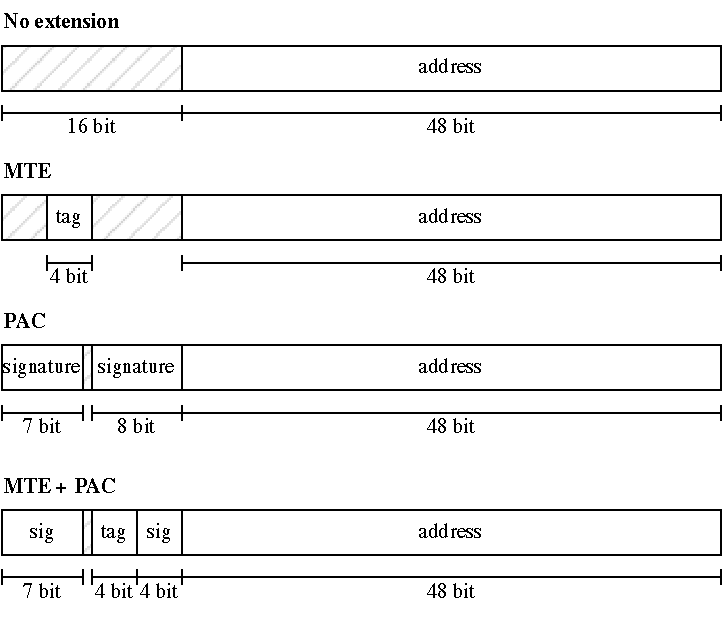
\includegraphics[scale=1]{figures/build/pointer-aarch64}
    \caption{Pointer layout on aarch64 in Linux with and without \ac{MTE} and \ac{PAC} enabled.}
    \label{fig:aarch64-pointer}
\end{figure}

In \cref{fig:aarch64-pointer}, we show the layout of pointer bits used for address translation in aarch64, the 64-bit variant of the ArmV8 instruction set~\cite{ARMA2024Arch64}, when running on Linux.
Only 48 out of the available 64\ bits are used to address memory, while the remaining bits are set to either 0 or 1 to differentiate between kernel and userspace addresses but are unused for further address translation.
Hardware extensions such as \ac{TBI}, \ac{MTE} (\cref{subsec:mte}), or \ac{PAC} (\cref{subsec:pac}) utilize those unused bits to store metadata.

\subsection{Memory Tagging Extension (MTE)}
\label{subsec:mte}

ARMs \Ac{MTE}, available from ArmV8.5, provides a building block to prevent spatial and temporal memory safety violations~\cite{ARM2019MTE}.
\Ac{MTE} implements a lock-and-key mechanism where memory regions can be tagged with one of 16 distinct tags, and memory access is only allowed using pointers with the corresponding keys.

The locking mechanism is implemented by storing a 4-bit tag in bits 56--59 of an address (referred to as the logical tag).
Accordingly, a tag is assigned to memory with a granularity of 16\,bytes (referred to as the allocation tag).

On Linux, each process can configure \ac{MTE} by switching between the following modes:
\begin{itemize}
    \item \textbf{Disabled:} \ac{MTE} is disabled, and no tag checks are performed.
    \item \textbf{Synchronous:}
    Tag mismatches cause a hardware fault on instruction retirement, and a segmentation fault is delivered to the application.
    The faulting instruction cannot read the affected memory location, or the update is not observable in the case of writes.
    \item \textbf{Asynchronous:}
    Tag mismatches do not cause an immediate hardware fault.
    Instructions may be able to read the memory location regardless of tag mismatches, or the update may be observable in the case of writes.
    The fault is delivered after the instruction has retired in the form of a CPU flag.
    The kernel will check this flag at the next context switch and deliver a segmentation fault to the application.
\end{itemize}

\subsubsection{Temporal and Spatial Memory Safety}

\begin{figure}[t]
    \centering
    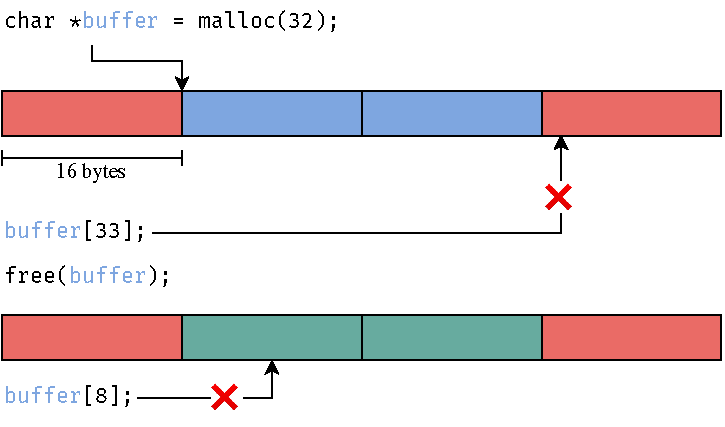
\includegraphics[scale=1]{figures/build/mte}
    \caption{Example of a heap allocation protected by \ac{MTE}.}
    \label{fig:mte}
\end{figure}

\Ac{MTE} can provide spatial memory safety by assigning different tags to adjacent regions and temporal memory safety by retagging freed memory.
An example can be seen in \cref{fig:mte}.

\subsection{Pointer Authentication (PAC)}
\label{subsec:pac}

\Ac{PAC}~\cite{Qualcomm2017PointerAuth} introduces primitives to prevent attackers from modifying pointers stored in memory.
The extension provides three instructions for signing pointers, authenticating, or stripping the signature from pointers.
\ac{PAC} places the signature in the upper 16 bits of pointers, with the exact layout dependent on the operating system, hardware, and other factors, such as if \ac{MTE} is enabled.
The signature can be between 7 and 16\,bits long.

Signed pointers are invalid and cannot be used to address memory.
They are created using the \texttt{pac*} instructions.
Before being used, the signature needs to be removed.
This happens either with the \texttt{aut*} instructions, which remove the signature if it is valid or produce a pointer that will trap when used if the signature does not match the address.
The extension provides \texttt{strip} instructions to remove the signature regardless of whether it is valid or not.

\paragraph{} \ac{MTE} and \ac{PAC} can be combined at the cost of bits available for the \ac{PAC} signature.
The exact layout of the \ac{PAC} signature varies depending on the system.
On Linux, bits 56--59 are used for \ac{MTE} while bits 63--60 and 54--49 are used for \ac{PAC} (see \cref{fig:aarch64-pointer}).
The remaining bit 55 differentiates between lower and upper (kernel- and userspace) addresses.

    \chapter{Motivation}
\label{ch:motivation}

While WebAssembly provides strong safety and security guarantees, as discussed in \cref{sec:wasm}, these mainly guarantee safety for the host, not the program itself.
In~\cite{lehmann2020everything}, \citeauthor*{lehmann2020everything} show that while some attack surfaces, such as injecting shellcode or jumping to arbitrary addresses, are mitigated by the design of WebAssembly, others, such as buffer overflows or write accesses to static, read-only data is possible and being used to exploit programs running in the wild.
These need to be mitigated at the language level by rewriting software in a safe language such as Rust, manually inserting bounds checks, which is error-prone, or inserting checks using the compiler and sanitizing the code.

Additionally, bugs like {CVE-2023-4863}~\cite{CVE-2023-4863} continue to be exploited, showing that memory safety is not a solved problem.
While they do not escape the WebAssembly sandbox, they pose a security risk to the programs themselves.
In C, the use of unsafe primitives or bugs, such as missing bounds checks, can be exploited by the attackers, e.g., by overwriting a variable to elevate their privileges.
In \cref{fig:vulnerable-overflow}, the lack of bounds checks allows an attacker controlling the variable \texttt{input} to write beyond the allocation of \texttt{buf} and overwrite \texttt{str}.

\begin{figure}[h]
    \centering
    \begin{lstlisting}[frame=h,style=customc,label={lst:vulnerable-overflow}]
void foo(char *input) {
    char buf[32];
    const char str = "Hello, World!";
    strcpy(buf, input);
}
    \end{lstlisting}
    \caption{Vulnerable overflow}
    \label{fig:vulnerable-overflow}
\end{figure}

To contain potentially malicious programs within their sandbox, several different techniques may be used, as discussed in \cref{subsec:webassembly-sandbox}.
Most implementations rely on virtual memory and guard pages to contain memory access when possible.
However, in cases where virtual memory cannot be used, e.g., when running 64\,bit WebAssembly programs, the engine needs to fall back to software-based bounds checks, bringing a significant performance penalty.
In our measurements, switching to 64\,bit \ac{WASM} resulted in a roughly 6-8\,\% overhead on out-of-order CPUs, which can speculate bounds checks, and \todo{x}\,\% overhead on in-order CPUs (see detailed evaluation in \cref{sec:performance-overheads}).
The fallback to software-based bounds checks is thus especially painful when running on low-power in-order cores when running 64\,bit \ac{WASM} or in environments without an operating system, such as embedded devices.


    \chapter{Overview}
\label{ch:overview}

In this thesis, we present a design for an extension that enhances memory safety in \ac{WASM} built on top of the \ac{WASM} 64-bit memory proposal\footnote{\url{https://github.com/WebAssembly/memory64}}.
The extension is created to be minimally invasive and implementable using various techniques, including hardware extensions such as \ac{MTE} or \ac{PAC}, capability-based architectures like \ac{CHERI}~\cite{woodruff2014cheri}, or software-based solutions similar to \ac{ASAN}~\cite{serebryany2012addresssanitizer} or \ac{HWASAN}~\cite{serebryany2018memory} (see \cref{ch:design}).


\begin{figure}[ht]
    \centering
    % not the best name lmao
    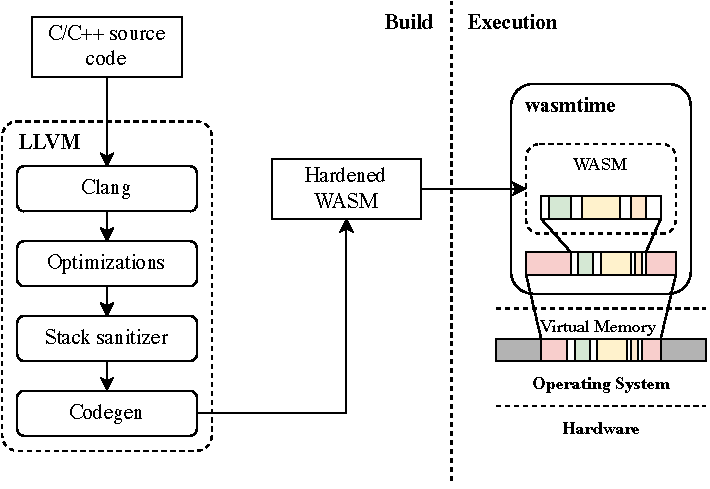
\includegraphics{figures/build/overview-simple}
    \caption{Overview of the prototype implemented in this thesis.}
    \label{fig:system-overview}
\end{figure}

In \cref{fig:system-overview} we present our prototype of this design.
Unmodified C/C++ source code is compiled using LLVM~\cite{lattner2004llvm}, where we implement a sanitizer that identifies and hardens stack allocations, along with a modified standard library based on \ac{WASI} that protects heap allocations.
LLVM then generates hardened \ac{WASM} binaries that can be run in wasmtime\footnote{\url{https://wasmtime.dev/}}.
We modify wasmtime to process our \ac{WASM} extension and implement it using \ac{MTE}.

Additionally, we explore and implement a technique to efficiently sandbox \ac{WASM} programs using \ac{MTE}, eliminating expensive software-based bounds checks required for 64\,bit \ac{WASM} programs.
This technique can be combined with the \ac{MTE}-based memory safety implementation.

We analyze and benchmark various aspects of our implementation, including 32\,bit and 64\,bit \ac{WASM}, and the \ac{MTE} implementation on real hardware (see \cref{ch:eval}).

    \chapter{Design}
\label{ch:design}

This chapter defines our threat model, \ac{WASM} extension, and design to provide memory safety for programs compiled to \ac{WASM}.

\section{Threat Model}
\label{sec:threat-model}

In our threat model (\cref{fig:threat-model}), we differentiate between two aspects of memory safety:

\begin{figure}
    \centering
    \begin{subfigure}[T]{0.45\textwidth}
        \centering
        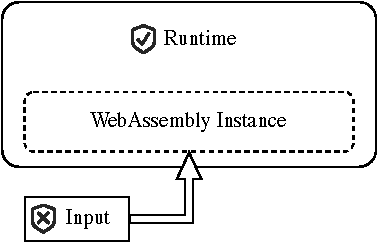
\includegraphics{figures/build/wasm-internal-mem-safety}
        \caption{Internal memory safety.}
        \label{fig:internal-mem-safety}
    \end{subfigure}
    \hfill
    \begin{subfigure}[T]{0.45\textwidth}
        \centering
        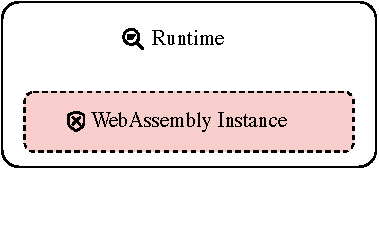
\includegraphics{figures/build/wasm-external-mem-safety}
        \hspace{\fill}
        \caption{External memory safety.}
        \label{fig:external-mem-safety}
    \end{subfigure}
    \caption{Threat model for internal and external memory safety.}
    \label{fig:threat-model}
\end{figure}

\begin{description}
    \item[Internal Memory Safety:] Ensures memory safety within the boundaries of a sandbox.
    Our point of view is from within a WebAssembly instance, we trust the runtime (and the host we are running on), but we do not trust external input (\cref{fig:internal-mem-safety}).
    \item[External Memory Safety:] Maintains the memory safety of the sandbox itself against potentially malicious programs.
    Our point of view is from the runtime; we trust the platform we are running on, but not the WebAssembly programs we are executing (\cref{fig:external-mem-safety}).
\end{description}

\subsection{Internal Memory Safety}
\label{subsec:internal-memory-safety}
For internal memory safety, the program within the sandbox and its runtime, including its compiler, are considered trusted and assumed to be bug-free.
Untrusted input (e.g., network data, file reads) originates from outside the sandbox and may be controlled by an attacker.
This model mirrors the threat environment of a standard non-\ac{WASM} program.
Potential threats include:

\begin{itemize}
    \item \textbf{Buffer overflows:} Attempts to access memory beyond allocated buffer boundaries.
    \item \textbf{Use-after-free:} Attempts to access deallocated memory.
\end{itemize}

\noindent
As discussed in \cref{sec:wasm}, WebAssembly's design inherently mitigates some threats common in non-\ac{WASM} environments, so we will not consider the following vectors:

\begin{itemize}
    \item \textbf{Return-oriented attacks:} {\ac{WASM}'s} structured control flow constructs prevent arbitrary code execution through stack manipulation.
    \item \textbf{Calling unknown function pointers:} Function tables enforce a strict mechanism for function calls, ensuring the integrity of call targets.
\end{itemize}

\subsection{External Memory Safety}
\label{subsec:external-memory-safety}

For external memory safety, we focus on the security of the sandbox.
Threats originate from running untrusted programs, which may be adversarial or buggy.

\begin{itemize}
    \item \textbf{Sandbox escapes:} Attempts to break out of the sandbox's restrictions and access host resources.
    \item \textbf{Side-channel attacks:} Exploiting timing differences or resource usage patterns to infer sensitive information.
\end{itemize}

\noindent
We assume that the operating system and underlying target architecture are free of bugs that malicious targets might exploit.
This does not include assumptions about potential spectre-like~\cite{kocher2020spectre} attacks.
The compiler needs to ensure that bounds checks are guarded against side-channel attacks.

Additionally, we do not consider exploits of the program running in the sandbox as vulnerabilities as long as they stay contained in the sandbox.

\section{Overview}
\label{sec:overview}

\begin{figure*}[t]
    \centering
    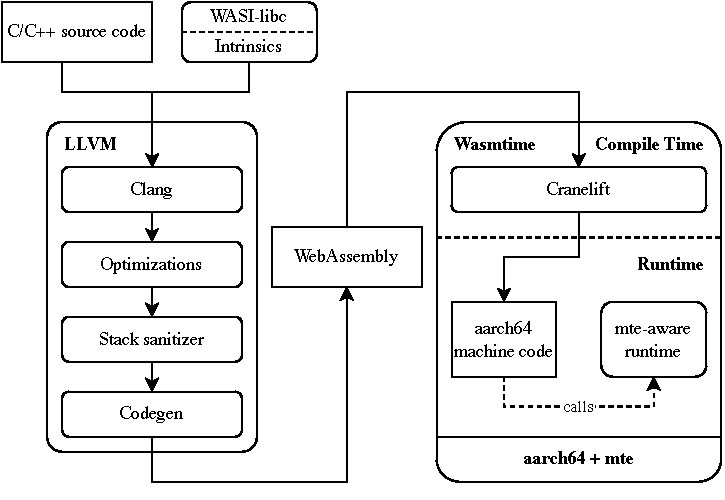
\includegraphics{figures/build/overview}
    \caption{Overview of the compilation and execution workflow.}
    \label{fig:overview}
\end{figure*}

Figure~\ref{fig:overview} presents an overview of our prototype.

At build time, the unmodified C/C++ sources and a modified version of libc are compiled using LLVM~\cite{lattner2004llvm}.
After optimizations, a stack sanitizer analyzes all functions and inserts instrumentation as necessary.
LLVM's backend then generates WebAssembly binaries that can be deployed and executed on various devices.

\section{WebAssembly Extension}
\label{sec:wasm-extension}

We designed an extension to WebAssembly that provides primitives to the modified standard library and the stack sanitizer to guarantee memory safety for selected allocations.
Our extension builds on wasm64, the 64\,bit variant of WebAssembly.
We choose wasm64, because it uses a 64\,bit integer index type, with 48 of those bits used to index memory.
This allows us to allocate and store up to 16 bits of metadata per pointer.

For our extension, we introduce the notion of abstract segments and tagged pointers.
We introduce three new instructions that allow the creation of abstract segments and tagged pointers from raw pointers.
These pointers carry provenance and can only access the segment they were created with.
Conversely, segments can only be accessed by the tagged pointer created with them rather than with raw indices without provenance.

\begin{equation*}
    \text{(new instructions) } e \Coloneqq \textbf{segment.new} \mid \textbf{segment.set\_tag} \mid \textbf{segment.free}
\end{equation*}

\paragraph{}
In the following paragraph, we describe the new instructions in detail.

\begin{description}
    \item[\texttt{segment.new}:] Create a new, zeroed memory segment.
    This instruction takes two arguments: a memory index and a size.
    The instruction generates a new tag, assigns it to the piece of memory, and returns a tagged pointer that can be used to access the segment.
    \item[\texttt{segment.set\_tag}:] This instruction takes a memory index, a length, and a tagged pointer and applies the tag from the tagged pointer to the memory segment located at the index with the passed length.
    This can be used to move ownership from one segment to another or to merge segments.
    \item[\texttt{segment.free}:] This instruction invalidates a segment by tagging the segment with a new, implementation-defined tag.
    This instruction takes two arguments: a memory index and a length.
    After this instruction, the tagged pointer being used to access the segment is no longer valid, and accessing the segment through it will result in a trap.
\end{description}

We also modify the semantics of existing load and store instructions.
They still take an integer as an index, but we introduce provenance to integers, which we can track at runtime using the unused 16 upper bits in pointers.
If a segment is accessed, the runtime will check that the tagged pointer is allowed to access the segment, i.e., the metadata matches the metadata created by the \texttt{segment.new} instruction.
If this is not the case, the runtime throws a trap.

At startup, the linear memory consists of a single segment that can be accessed using untagged indices, allowing unmodified code to run under our new semantics without modifications.
This design choice also allows the gradual integration of safety primitives into specific parts of WebAssembly applications where enhanced security is required.
For instance, it enables the introduction of a hardened malloc implementation, which prevents spatial and temporal safety bugs for heap-allocated memory.
Additionally, we can analyze stack allocations to only harden those accessed using untrusted indices or escape our analysis, e.g., by taking their address and passing it to another function.

\paragraph{Alignment}
All segments are aligned to 16 bytes, corresponding to the alignment of \ac{MTE} (see \cref{subsec:mte}).
This is an implementation choice that may be changed once we support additional implementations.
More details can be found in \cref{sec:future-work}.

\subsection{Typing Rules}
\label{subsec:typing}

In \cref{fig:typing-rules}, we extend the typing rules in the \ac{WASM} paper~\cite{haas2017bringing} in the notation of \citeauthor*{pierce2002types}~\cite{pierce2002types}.
The rules are of the form of $C \vdash e : \mathit{tf}$.
An instruction $e$ is valid under the context $C$, with $C_\text{memory}$ being used to access a context component, such as the memory.
The rule $C_\text{memory} = n$ ensures that the instruction can only be used when a memory is declared.
The rule $2^a=16$ ensures the alignment is 16\,bytes, as described in the previous section.
The type $\mathit{tf} = t_1^* \rightarrow t_2^*$ describes how the instruction manipulates the operand stack.
The instruction $e$ expects an operand stack where it pops off $t_1^*$ and pushes $t_2^*$.

\begin{figure}[t]
    \begin{prooftree}
        \AxiomC{$C_{\text{memory}} = n$}
        \AxiomC{$2^a=16$}
        \BinaryInfC{$C \vdash \textbf{segment.new}\ a\ o : \text{i64}\ \text{i64} \rightarrow \text{i64}$}
    \end{prooftree}
    \begin{prooftree}
        \AxiomC{$C_{\text{memory}} = n$}
        \AxiomC{$2^a=16$}
        \BinaryInfC{$C \vdash \textbf{segment.set\_tag}\ a\ o : \text{i64}\ \text{i64}\ \text{i64} \rightarrow \epsilon$}
    \end{prooftree}
    \begin{prooftree}
        \AxiomC{$C_{\text{memory}} = n$}
        \AxiomC{$2^a=16$}
        \BinaryInfC{$C \vdash \textbf{segment.free}\ a\ o : \text{i64}\ \text{i64} \rightarrow \epsilon$}
    \end{prooftree}
    \caption{Typing rules of the new instructions. For the definition of context $C$, see the \ac{WASM} paper~\cite{haas2017bringing}.}
    \label{fig:typing-rules}
\end{figure}

\subsection{Small-Step Reduction Rules}
\label{subsec:small-step-reduction-rules}

In \cref{fig:smallstep-rules}, we extend the small-step reduction rules from the WASM paper~\cite{haas2017bringing} using the notation established by \citeauthor*{plotkin1981structural}~\cite{plotkin1981structural}.
The lower portion of  \cref{fig:smallstep-rules} presents new tag-aware load/store rules that take precedence over the existing ones and new rules for the introduced instructions.

To signal a trap, we reuse operators from the original WASM rules, including the \textbf{trap} operator.
The state, $s$, is augmented with a storage mechanism that assigns a tag $t$, to each memory byte.
We use the following notation:

\begin{itemize}
    \item $s_{\text{tag}}(i, \mathit{addr}, \mathit{len})$: Extracts tags for a memory region accessed by instruction $i$ at address $\mathit{addr}$ with length $\mathit{len}$.
    \item $s' = s\ \text{with}\ \text{tag}(i, \mathit{addr}, \mathit{len}) = t$: Updates the state with new tags for the memory region at address $\mathit{addr}$ with length $\mathit{len}$.
    \item $t = \text{tag}(\mathit{pointer})$: Extracts the tag from a tagged pointer.
    \item $t' = \text{new\_tag}(t)$: Creates a tagged pointer $t'$ from an untagged pointer $t$ to be used for a new segment.
    \item $t' = \text{free\_tag}(t)$: Creates a tagged pointer $t'$ for the purpose of freeing a segment.
\end{itemize}

\noindent
\Cref{fig:smallstep-rules} highlights the added and modified components in the rules.
The added load/store rules, specified in \cref{eq:smallstep-1,eq:smallstep-2}, enforce trapping on tag mismatches.
The rules for executing the new instructions, which modify the state by setting tags, are presented in \cref{eq:smallstep-3,eq:smallstep-4,eq:smallstep-5}.
Each reduction rule is depicted with the operand stack's top and state $s$ on the left-hand side, representing the pre-execution state, and the resulting stack and state after the execution of instruction $i$ on the right-hand side.

\begin{figure}[t]
    \begin{align*}
        \text{(store)}\ s &\Coloneqq \{\dots, \text{tag}\ \mathit{taginst}^*\} \\
        \mathit{taginst} &\Coloneqq b^*
    \end{align*}
    \begin{align}
        s;(\textbf{i64.const}\ k);(t\textbf{.load}\ a\ o)\ &\hookrightarrow_i\ \textbf{trap} \label{eq:smallstep-1}
        \shortintertext{\hfill $\text{if}\ s_\text{tag}(i, k + o,\lvert t \rvert) \neq \text{tag}(k)$\vskip1em}
        s;(\textbf{i64.const}\ k);(t\textbf{.const}\ c);(t\textbf{.store}\ a\ o)\ &\hookrightarrow_i\ \textbf{trap} \label{eq:smallstep-2}
        \shortintertext{\hfill $\text{if}\ s_\text{tag}(i, k + o,\lvert t \rvert) \neq \text{tag}(k)$\vskip1em}
        s;(\textbf{i64.const}\ k);(\textbf{i64.const}\ s);(\textbf{segment.new})\ &\hookrightarrow_i\ s';(\textbf{i64.const}\ t) \label{eq:smallstep-3}
        \shortintertext{\hfill $\text{if}\ t = \text{new\_tag}(k) \land s' = s\ \text{with}\ \text{tag}(i, k, s) = t$\vskip1em}
        s;(\textbf{i64.const}\ k);(\textbf{i64.const}\ t);(\textbf{i64.const}\ s);(\textbf{segment.set\_tag})\ &\hookrightarrow_i\ s' \label{eq:smallstep-4}
        \shortintertext{\hfill $\text{if}\ s' = s\ \text{with}\ \text{tag}(i, k, s) = t$\vskip1em}
        s;(\textbf{i64.const}\ k);(\textbf{i64.const}\ s);(\textbf{segment.free})\ &\hookrightarrow_i\ s' \label{eq:smallstep-5}
        \shortintertext{\hfill $\text{if}\ t = \text{free\_tag}(k) \land s' = s\ \text{with}\ \text{tag}(i, k, s) = t$} \notag
    \end{align}
    \caption{Small-step reduction rules of the new instructions and added rules for load/stores. See the \ac{WASM} paper~\cite{haas2017bringing} for the definitions of all rules and auxiliary constructs.}
    \label{fig:smallstep-rules}
\end{figure}

\subsection{Example}
\label{subsec:example}

We will demonstrate our \ac{WASM} extension using the C snippet in \cref{lst:wasm-example-c}, which allocates 64 bytes on the stack.

\begin{lstfloat}
    \begin{lstlisting}[frame=h,style=customc,
        label={lst:wasm-example-c-inner}]
    void foo() {
        char buf[64];
        // ...
        return;
    }
    \end{lstlisting}
    \caption{Example of a C program allocating 64 bytes on the stack.}
    \label{lst:wasm-example-c}
\end{lstfloat}

\noindent
This requires the compiler to instrument the stack allocation, create a new segment, and free the segment before returning to the caller, i.e., giving ownership of the stack slot back to the stack frame, as demonstrated in \cref{lst:wasm-example}.

\begin{lstfloat}
    \begin{lstlisting}[frame=h,style=customwasm,
        label={lst:wasm-example-inner},escapechar=|]
    ;; Allocate space on the stack
    global.get $__stack_pointer|\label{line:alloc-1}|
    i64.const 64|\label{line:alloc-2}|
    i64.sub|\label{line:alloc-3}|
    global.tee $__stack_pointer|\label{line:alloc-4}|

    ;; create a seg||ment
    i64.const 64|\label{line:segment-new-1}|
    segment.new|\label{line:segment-new-2}|
    local.set $buf|\label{line:segment-new-3}|

    ;; ...

    ;; retag with stack pointer tag
    local.get $buf|\label{line:segment-set-tag-1}|
    global.get $__stack_pointer|\label{line:segment-set-tag-2}|
    i64.const 64|\label{line:segment-set-tag-3}|
    segment.set_tag|\label{line:segment-set-tag-4}|

    ;; reset stack pointer
    global.get $__stack_pointer|\label{line:reset-sp-1}|
    i64.const 64|\label{line:reset-sp-2}|
    i64.sub|\label{line:reset-sp-3}|
    global.set $__stack_pointer|\label{line:reset-sp-4}|
    \end{lstlisting}
    \caption{Generated \ac{WASM} for code from \cref{lst:wasm-example-c}.}
    \label{lst:wasm-example}
\end{lstfloat}

The compiler allocates the slot for \texttt{buf} on the stack, decrementing the global \texttt{\$\_\_stack\_pointer} acting as the stack pointer (\cref{line:alloc-1,line:alloc-2,line:alloc-3,line:alloc-4}).
Then, a new segment of size 64 is created, and the tagged pointer to it is stored in the local \lstinline[style=customwasm]{$buf} ((\cref{line:segment-new-1,line:segment-new-2,line:segment-new-3})).
Before returning, the segment is retagged using the stack pointers tag, i.e., restoring the previous tag and allowing access through the stack pointer (\cref{line:segment-set-tag-1,line:segment-set-tag-2,line:segment-set-tag-3,line:segment-set-tag-4}).
Then, the stack pointer is reset, freeing the stack frame (\cref{line:reset-sp-1,line:reset-sp-2,line:reset-sp-3,line:reset-sp-4}).

\subsection{Heap Safety}
\label{subsec:heap-safety}

The memory allocator needs to be aware of segments to provide heap safety.
When allocating memory, it aligns the requested size to 16 bytes, creates a segment, and returns the corresponding tagged pointer.
This prevents overflows from corrupting allocator metadata or other memory segments.
A modified allocator implementation looks conceptually similar to the snippet in \cref{lst:heap-allocator-example}.

\begin{lstfloat}
    \begin{lstlisting}[frame=h,style=customc,
        label={lst:heap-allocator-example-inner}]
    void *malloc(size_t length) {
        void *chunk = /* perform allocation */;
        return __builtin_wasm_segment_new(chunk, length);
    }
    \end{lstlisting}
    \caption{Example of a malloc implementation utilizing the memory safety extension.}
    \label{lst:heap-allocator-example}
\end{lstfloat}

\noindent
When compiled to \ac{WASM}, we see just three new instructions added to the generated code (\cref{line:segment-new-heap-1,line:segment-new-heap-2,line:segment-new-heap-3}).
This proves that our extension is minimally invasive, as the calling code does not need to be changed and will continue to work as-is.
Similarly, when freeing or reallocating memory, the allocator needs to ensure that the no longer valid memory is retagged.

\begin{lstfloat}
    \begin{lstlisting}[frame=h,style=customwasm,
        label={lst:wasm-allocator-example-inner},escapechar=|]
    (func $malloc (param $length i64) (result i64) (local $chunk)
        ;; perform allocation and place the res||ult in $chunk
        ;; ...

        ;; create a seg||ment
        local.get $chunk|\label{line:segment-new-heap-1}|
        local.get $length|\label{line:segment-new-heap-2}|
        segment.new|\label{line:segment-new-heap-3}|
        ;; implicit ret||urn
    )
    \end{lstlisting}
    \caption{Generated \ac{WASM} for code from \cref{lst:heap-allocator-example}.}
    \label{lst:wasm-allocator-example}
\end{lstfloat}

\subsection{Stack Safety}
\label{subsec:stack-safety}

For stack safety, we create segments from stack slots when entering a function.
Before returning, all stack slots are untagged and reassigned to the stack frame.
This allows other functions to use the memory and prevents stack slots from being accessed after returning from a function.

However, only some stack allocations need to be turned into segments.
We can omit allocations that do not escape or are only accessed using statically verifiable indices.
Creating segments for these would result in excessive runtime and memory overhead, as each allocation would need to be aligned to 16\,bytes and processed when entering and returning from a function.

To address this, we design an algorithm (\cref{fig:stack-safety-pseudo}) that identifies safe memory regions within the stack that do not require protection, thus avoiding creating segments for the slots mentioned above.
Below, we present a simplified version of our algorithm.
We iterate over all stack allocations and check if the allocation (a) escapes the function or (b) is indexed into using an unsafe \ac{GEP} instruction.

\begin{figure}
    \begin{algorithmic}
        \State $allocsToInstrument \gets \emptyset$
        \For{$alloc \in allocations$}
            \If{escapes($alloc$)}
                \State $allocsToInstrument \gets allocsToInstrument \cup \{\,alloc\,\}$
            \ElsIf{isUsedByUnsafeGEP($alloc$)}
            \State $allocsToInstrument \gets allocsToInstrument \cup \{\,alloc\,\}$
            \EndIf
        \EndFor

        \For{$alloc \in allocsToInstrument$}
            \State insertTaggingCode($alloc$)
            \State insertUntaggingCode($alloc$)
        \EndFor
    \end{algorithmic}
    \caption{Algorithm to detect and harden safe and unsafe stack allocations.}
    \label{fig:stack-safety-pseudo}
\end{figure}

\subsection{Example}
\label{subsec:example2}

\begin{lstfloat}
    \begin{lstlisting}[frame=h,style=customc,
        label={lst:stack-safety-inner},escapechar=|]
    char foo(int index) {
      int i = 0; // safe|\label{line:ex-i}|
      int bytes_read = 0; // unsafe|\label{line:ex-bytes-read}|
      char buf[32]; // unsafe|\label{line:ex-buf}|
      read_input(buf, &bytes_read);|\label{line:ex-escape}|
      return buf[index];|\label{line:ex-access}|
    }

    char *bar() {
        char buf[32]; // unsafe
        return buf;|\label{line:ex-ret}|
    }
    \end{lstlisting}
    \caption{Example code for safe and unsafe stack slots.}
    \label{lst:stack-safety}
\end{lstfloat}

We demonstrate the algorithm using the function in \cref{lst:stack-safety}.
In the code example, \texttt{i} (\cref{line:ex-i}) is safe, as its address is not used in a potentially unsafe address computation and does not escape.
The variables \texttt{bytes\_read} and \texttt{buf} (\cref{line:ex-bytes-read,line:ex-buf}) are deemed unsafe as their address escapes (\cref{line:ex-escape}).
Additionally, \texttt{buf} is accessed using an untrusted index (\cref{line:ex-access}).

\noindent
In function \texttt{bar}, \texttt{buf} also needs to be instrumented as it escapes: the pointer to it is returned to the caller (\cref{line:ex-ret}).
Any attempt to dereference the value returned by \texttt{bar} is undefined behavior and will be caught by our instrumentation, preventing difficult-to-debug bugs or potential vulnerabilities.

\noindent
This algorithm effectively balances the need for stack safety with performance and memory efficiency constraints.

    \chapter{Implementation}
\label{ch:implementation}

Our implementation of \projectname{} is integrated into the LLVM framework, wasi-libc, and the wasmtime WebAssembly runtime.
The following sections detail the specific modifications and extensions we made to each component, as well as some of the implementation choices and details to tackle specific problems.

\section{LLVM}
\label{sec:llvm}

We chose LLVM as our compiler from C/C++ to WebAssembly.
To be able to compile to our memory safety extension, we modified the WebAssembly backend to add support for our new instructions, allowing LLVM to emit our extension in both bytecode and text format.

\subsection{LLVM IR}
\label{subsec:llvm-ir}

In the middle end, we introduced three new intrinsic functions that correspond and are lowered to our \ac{WASM} instructions by the backend.
\begin{itemize}
  \item \lstinline[style=customc,language=llvm]{ptr @llvm.wasm.segment.new(ptr, i64);}
  \item \lstinline[style=customc,language=llvm]{void @llvm.wasm.segment.set_tag(ptr, ptr, i64);}
  \item \lstinline[style=customc,language=llvm]{void @llvm.wasm.segment.free(ptr, i64);}
\end{itemize}
Calls to these intrinsic functions can be inserted by the frontend or a sanitizer pass.
A function that allocates 32 bytes on the stack might be lowered to the following IR:

\begin{lstlisting}[frame=h,style=customc,
    label={lst:llvm-intrinsics},language=llvm]
define hidden signext void @foo(i32 %index) {
entry:
  %arr = alloca [32 x i8], align 16
  ; create a new segment
  %1 = call ptr @llvm.wasm.segment.new(ptr %arr, i64 32)

  ; do some work

  ; return ownership of segment to tag
  call void @llvm.wasm.segment.set.tag(ptr %1, ptr %arr, i64 32)
  ret void
}
\end{lstlisting}

\subsection{LLVM Sanitizer Pass}
\label{subsec:llvm-sanitizer-pass}

In LLVM, we introduced a WASM-specific sanitizer pass that can be enabled via a compiler flag, designed to provide memory safety for stack allocations when compiling to WebAssembly.
This sanitizer analyzes functions for stack allocations and applies padding and tagging to them, as discussed in \cref{subsec:stack-safety}.
The pass runs after all optimizations, ensuring we do not block passes that might remove stack allocations, such as \texttt{mem2reg}.

As WebAssembly does not support exceptions or C-style long jumps, we do not have to handle these special cases, which have been proven to be tricky to implement with tagged memory in the past.

\subsection{C extension}
\label{subsec:c-extension}

To be able to create and manipulate segments manually, e.g.\ to build a segment-aware memory allocator, we need to expose some primitives to C.
We do this by creating three builtin functions in clang that are lowered to intrinsic calls in LLVM.

\begin{itemize}
  \item \lstinline[style=customc]{void *__builtin_wasm_segment_new(void *, unsigned long);}
  \item \lstinline[style=customc]{void __builtin_wasm_segment_set_tag(void *, void *, unsigned long);}
  \item \lstinline[style=customc]{void __builtin_wasm_segment_free(void *, unsigned long);}
\end{itemize}

The functions can be used as regular functions in C code, e.g.:

\begin{lstlisting}[frame=h,style=customc,
  label={lst:builtin-functions}]
void *my_malloc(unsigned long size) {
  void *memory = malloc(size);
  return __builtin_wasm_segment_new(memory, size);
}
\end{lstlisting}

\section{WASI Libc Modifications}
\label{sec:wasi-libc}

To allow us to run applications relying on libc on wasm64, we had to port \ac{WASI} and wasi-libc to wasm64.
This mainly consisted of mechanical work, changing size and pointer types from 32 to 64\,bits.

To provide memory safety for heap allocations, we modified dlmalloc, the default allocator in wasi-libc.
This consisted of inserting calls to our builtin functions as necessary, creating memory segments and returning tagged pointers instead of returning the pointer to the just allocated piece of memory.
This protects both allocator metadata and adjacent allocations from being accessed or modified through heap overflows.
The allocator also ensures that segments are freed when freeing or reallocating memory, ensuring temporal safety.

\section{Wasmtime}
\label{sec:wasm-runtime}

As our runtime to build our prototype, we chose wasmtime\footnote{\url{https://wasmtime.dev/}}, a WebAssembly runtime with a focus speed and correctness, written in Rust, with its own optimizing compiler, cranelift\footnote{\url{https://cranelift.dev/}}, which also features its own \ac{IR}, \ac{CLIF}.

We modified wasmtime, as well as its supporting libraries, and extended it with support to parse and process the memory safety extension described in \cref{sec:wasm-extension}.
We added support for \ac{MTE} in the form of new instructions and lowering rules to cranelift, allowing wasmtime to generate \ac{MTE} instructions when compiling for a target that supports them.

By default, the memory is tagged with one of the tags described in \cref{tab:default-tag}.

\begin{table}
  \centering
  \begin{tabular}{c | c || c}
    \textbf{Memory Safety} & \textbf{MTE Sandboxing} & \textbf{Default Tag} \\
    \hline
    no & no & $t \in \{\,0\,\}$ \\
    yes & no & $t \in \{\,0\,\}$ \\
    yes & yes & $t \in \{\,1\,\}$ \\
    no & yes & $t \in \{\,1, \dots, 15\,\}$
  \end{tabular}
  \caption{Default tag $t$ for the linear memory}
  \label{tab:default-tag}
\end{table}

For \ac{MTE}, we store the logical tag directly in the \ac{WASM} index.
When assigning the allocation tag, however, we need to translate the index to an address.
Before assigning tags, we also need to perform explicit bounds checks, otherwise we would allow untrusted guest code to set arbitrary tags in the processes address space.
In the following paragraphs we will describe how we lower each of our instructions to an \ac{MTE} backend.

\paragraph{\lstinline[style=customwasm]{segment.new}} To create a new segment, we (1) check that the requested segment is inside the linear memory for the guest, (2) generate a random logical tag and insert it into the index, and (3) set the allocation tag for the segment.
This involves generating a loop that iterates over the size of the segment and setting the tag using \texttt{stzg}, which also zeroes the memory.

\paragraph{\lstinline[style=customwasm]{segment.set_tag}} To change ownership of a segment, we again (1) check that the requested segment is inside the linear memory for the guest and (2) set the new allocation tag for the segment.
Here we don't need to create a new, random tag, as we are passed a predefined tag.

\paragraph{\lstinline[style=customwasm]{segment.free}} To invalidate a segment, we (1) check that the requested segment is inside the linear memory for the guest and (2) set the default allocation tag for the segment.
The default tag depends on the configuration and can be taken from \cref{tab:default-tag}.

\paragraph{}
We have implemented a number of optimizations to ensure our generated code runs efficiently.
When setting the allocation tag for a segment, we generate a loop iterating over the size of the segment.
If the size of the loop is known at compile time, we unroll the loop to tag a larger amount of tags per iteration to avoid branch instructions.
This is only done up to a size of 160 bytes, which we chose as a tradeoff between code size and reducing the number of branch instructions executed.

\paragraph{}
If we are running the mode where both \ac{MTE} bounds checks and memory safety are enabled, we need a way to ensure only even tags are generated by instructions such as \texttt{irg} (\textbf{i}nsert \textbf{r}andom ta\textbf{g}) or \texttt{addg} (\textbf{add} ta\textbf{g}).
This can be either specified as an optional immediate to the instruction via an exclude mask, or through an include mask via a \texttt{prctl} call, which sets the corresponding register in kernel space.
We chose the latter option and set the include mask at startup time.

% TODO: write about MTE sync/async mode? We always use sync mode

    \chapter{Evaluation}
\label{ch:eval}


\section{Experimental Setup}\label{sec:experimental-setup}

We conduct our benchmarks on a Google Pixel 8 equipped with a Google Tensor G3 chip, comprising 1\,$\times$\,Cortex-X3 (2.91\,GHz), 4\,$\times$\,Cortex-A715 (2.37\,GHz), and 4\,$\times$\,Cortex-A510 (1.7\,GHz) cores, with \ac{MTE} enabled.
See \cref{tab:cores-comparison} for details on the benchmarked cores.
As of the time of writing, this is the sole commercially available device featuring \ac{MTE}.
To mitigate thermal throttling, we attach a cooling fan to the device.
Each performance test is run on each CPU type available on the Tensor G3 chip by pinning it to a single respective core.


\begin{table}[ht]
    \centering
    \small
    \caption{Comparison of the benchmarked cores.}
    \label{tab:cores-comparison}
    \begin{tabular}{l || l | l | l}
        \textbf{Spec}      & \textbf{Cortex-X3}    & \textbf{Cortex-A715} & \textbf{Cortex-A510} \\
        \hline
        Cores              & 1                     & 4                    & 4                    \\
        Pipeline           & in-order              & out-of-order         & out-of-order         \\
        Superscalar        & Yes                   & Yes                  & Yes                  \\
        Architecture       & ArmV9.2               & ArmV9.2              & ArmV9.2              \\
        Maxmimum Frequency & 2.91\,GHz             & 2.37\,GHz            & 1.7\,GHz             \\
        L1 I-Cache/D-Cache & 64\,KiB               & $32/64$\,KiB         & $32/64$\,KiB         \\
        L2 Cache           & 512\,KiB -- 1024\,KiB & 128\,KiB -- 512\,KiB & 128\,KiB -- 512\,KiB \\
        L3 Cache           & 512\,KiB -- 16\,MiB   & 512\,KiB -- 32\,Mib  & 256\,KiB -- 16\,Mib  \\
    \end{tabular}
\end{table}


\begin{table}[ht]
    \centering
    \small
    \caption{Runtime benchmarking configurations.}
    \label{tab:benchmark-variants}
    \begin{tabular}{c || c|c|c}
        \textbf{Variant} & \textbf{Pointer Width} & \textbf{Memory Safety} & \textbf{MTE Bounds Checks} \\
        \hline
        wasm32           & 32\,bit                & No                     & No                         \\
        wasm64           & 64\,bit                & No                     & No                         \\
        mem-safety       & 64\,bit                & Yes                    & No                         \\
        mte-bounds       & 64\,bit                & No                     & Yes                        \\
        combined         & 64\,bit                & Yes                    & Yes                        \\
    \end{tabular}
\end{table}

\noindent
We run the benchmarks from the PolyBench/C 3.2 suite~\cite{polybenchc}.


\section{Performance Overheads}
\label{sec:performance-overheads}

\begin{figure}[ht]
    \centering
    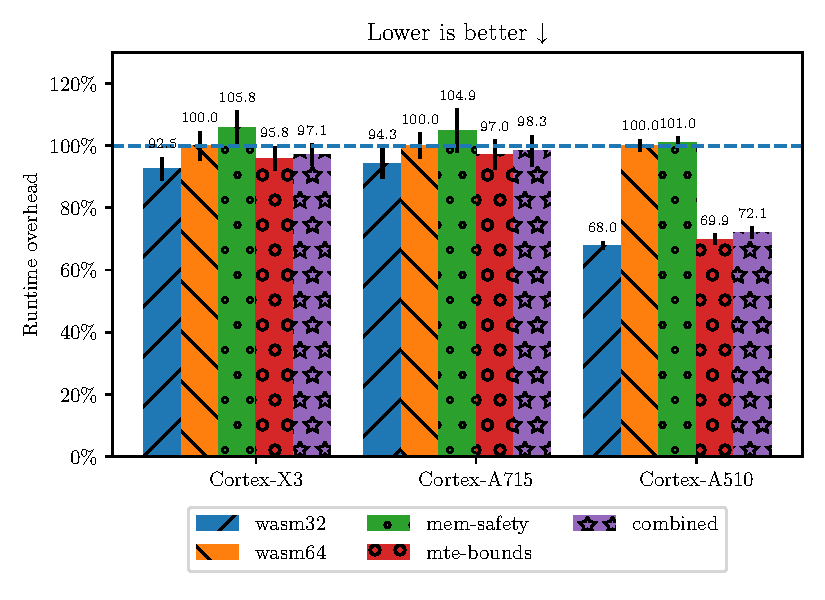
\includegraphics{plots/runtimes-all}
    \caption{PolyBench/C runtime overheads of different configurations described in \cref{tab:benchmark-variants}, normalized to wasm64.}
    \label{fig:runtime-overheads-combined}
\end{figure}

\Cref{fig:runtime-overheads-combined} illustrates the mean runtime overheads for PolyBench/C benchmarks for each CPU core available on the Tensor G3 chip.
Compared to wasm64, our memory safety extension has a mean overhead of 5.8\,\% and 4.9\,\% on the two out-of-order high-performance cores.
On the in-order Cortex-A510, we see an overhead of just 1.0\,\%.
Generally, we see that the overhead of bounds checks through the switch from wasm32 to wasm64 is lower on the out-of-order cores, as those can speculate on bounds checks, while the in-order cores cannot.
This also explains the low overhead of our memory safety extension on the in-order cores, as we spend more time doing bounds checks than on the in-order cores.

When we replace software-based bounds checks with \ac{MTE} bounds checks, we see the overhead largely disappearing.
The remaining overhead can be explained through (1) the natural overhead that enabling \ac{MTE} synchronous mode poses (see \cref{subsec:synchronous-and-asynchronous-mode}) and (2) the fact that the linear memory needs to be tagged on program startup.
This overhead is especially noticeable for short-running modules that require large amounts of linear memory.

Combining both \ac{MTE} bounds and \ac{MTE} memory safety, we see a slight increase from just \ac{MTE} bounds, which is smaller than the jump from wasm64 to memory safety.
The smaller increase is because we are not adding the \ac{MTE} overhead, as \ac{MTE} is already enabled.
The jump we see is the result of additional instructions tagging the segments.

We could decrease the overhead even further by switching to \ac{MTE} async mode, which is faster than sync mode (see \cref{subsec:synchronous-and-asynchronous-mode}).
However, this dramatically reduces the security guarantees provided by \ac{MTE}, as illegal writes and reads may become observable.
This disqualifies async \ac{MTE} for bounds checking of \ac{WASM} sandboxes, as attackers may carefully craft malicious code to escape their sandbox.
For the memory safety extension, users may decide the additional risk is worth the reduced overhead, e.g., when the memory safety extension is not used as a primary defense mechanism but as a second layer or to find bugs in the wild.


\section{Memory Overheads}\label{sec:memory-overheads}

Memory tagging incurs overhead, particularly for small allocations due to the 16-byte alignment required for \ac{MTE}.
Our measurements did not show a significant difference in maximum \ac{rss}.
This is because (1) safe allocations do not incur space overhead, and (2) for large allocations, the 16-byte alignment overhead is proportionally small.
The main overhead in \cref{fig:memory-overheads} is primarily due to the switch to wasm64, as pointer sizes are doubled.

\begin{figure*}[t]
    \centering
    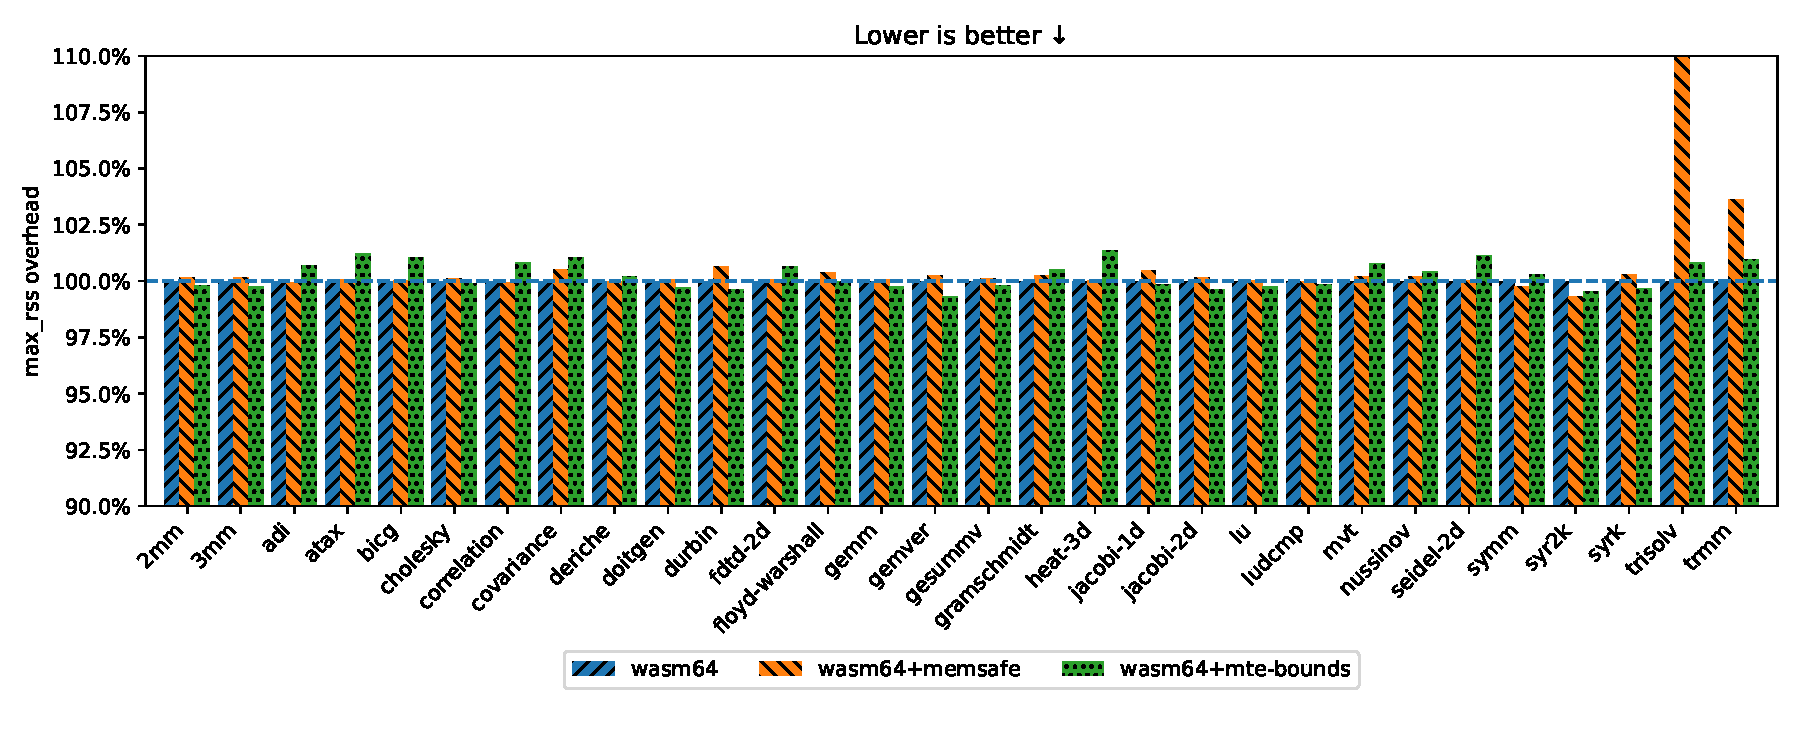
\includegraphics{plots/mem-overhead}
    \caption{PolyBench/C memory overheads of different configurations described in \cref{tab:benchmark-variants}, normalized to wasm64.}
    \label{fig:memory-overheads}
\end{figure*}


\section{Security Guarantees}\label{sec:security-guarantees}

We evaluate the security guarantees from the perspective of internal and external memory safety, as defined in \cref{sec:threat-model}.

\subsection{External Memory Safety}
\label{subsec:sec-guarantees-external-memory-safety}

Running with \ac{MTE} bounds checks, with \ac{MTE} being configured to run in synchronous mode, prevents programs from escaping their sandbox.
We prevent programs from forging tags by masking the respective tag bits before computing the effective address, as described in \cref{subsec:bounds-checks}.
Other defense mechanisms, such as structured control flow, the typed stack, and function calls through typed and checked tables, remain unchanged by our implementation.
However, we limit the number of sandboxes in one process to at most 15, which is required to assign a distinct tag to each sandbox.

Switching to async \ac{MTE} mode is not feasible to retain external memory safety, as memory accesses outside the sandbox may become observable to the \ac{WASM} module performing the illegal access and to other modules.

\subsection{Internal Memory Safety}
\label{subsec:sec-guarantees-internal-memory-safety}

Our choice to leverage \ac{MTE} allows for a low overhead, so this can be deployed in addition to testing using other mechanisms, such as \ac{ASAN}.
However, our approach does not provide complete memory safety for internal memory safety, as \ac{MTE} provides a limited number of tags and should be used as a secondary, not primary, defense mechanism to harden applications in the wild.
A tag collision means two memory regions could accidentally share the same tag, potentially leading to a missed security violation.
For example, if a buffer overflow writes slightly beyond its intended bounds, but the adjacent memory has the same tag, \ac{MTE} cannot detect the issue.

We can calculate the probability for a tag collision for $k=2$ random tags according to \cref{fig:tag-collision}, with $n=16$ available tags for \ac{MTE} bounds disabled (\cref{fig:tag-collision-16}) and $n=8$ for bounds enabled (\cref{fig:tag-collision-8}), as we reserve one bit for the bounds checking mechanism.

\begin{figure}[h]
    \centering
    \begin{subfigure}[T]{0.45\textwidth}
        \centering
        \begin{align*}
            V_{nr} &= \frac{n!}{(n - k)!} = 240 \\
            V_t &= n^k = 256 \\
            P(\text{c}) &= 1 - \frac{V_{nr}}{V_t} = 6.25\%
        \end{align*}
        \caption{Probability of a tag collision with $n=16$ and $k=2$.}
        \label{fig:tag-collision-16}
    \end{subfigure}
    \hfill
    \begin{subfigure}[T]{0.45\textwidth}
        \centering
        \begin{align*}
            V_{nr} &= \frac{n!}{(n - k)!} = 56 \\
            V_t &= n^k = 64 \\
            P(\text{c}) &= 1 - \frac{V_{nr}}{V_t} = 12.5\%
        \end{align*}
        \caption{Probability of a tag collision with $n=8$ and $k=2$.}
        \label{fig:tag-collision-8}
    \end{subfigure}
    \caption{Probabilities of tag collisions for random tags.}
    \label{fig:tag-collision}
\end{figure}

However, we ensure that adjacent allocations are always tagged with distinct tags and that memory is tagged with a new tag when it is freed, thus ensuring that spatial errors up to 16\,bytes and temporal errors until the subsequent allocation of a chunk of memory are always caught.


\section{MTE Performance evaluation}
\label{sec:mte-performance-evaluation}

We evaluated the performance of different characteristics of \ac{MTE} as implemented on the Tensor G3 chip.
All the programs used to measure results in this section are implemented in Rust and available on GitHub\footnote{\url{https://github.com/martin-fink/mte-stg-bench}}.
As our benchmarking library, we used criterion\footnote{\url{https://github.com/bheisler/criterion.rs}}.
After each benchmarking run, we let the device cool down for 30\,seconds to prevent throttling.
Additionally, we measure instruction throughput and latencies on all CPU cores.

\subsection{Instruction Latencies and Throughput}\label{subsec:instruction-latencies-and-throughput}

We evaluate instruction latencies and throughput in microbenchmarks executing 100,000,000 iterations of 100 instructions to minimize the effect of the looping code.
We use simpleperf\footnote{\url{https://android.googlesource.com/platform/system/extras/+/master/simpleperf/doc/README.md}} to measure CPU cycles of our benchmarking program\footnote{\url{https://github.com/martin-fink/mte-inst-cycles}}.
For each instruction, we measure three variants: (1) the baseline, which includes the startup, setup, and teardown of the benchmark, where no actual instructions are executed, (2) the latency test, where we measure instructions with data dependencies between them, and (3) the throughput test, where we measure instructions with no data dependencies.
We see the cycles and micro-ops per instruction in \cref{tab:instruction-latencies}.

We can make a few interesting observations:
\begin{itemize}
    \item For the set-tag instructions, Cortex-X3 has double the latency and half the throughput compared to Cortex-A720.
    \item On Cortex-A510, \texttt{st2g} has double the latency and half the throughput of \texttt{stg}, while also being the only one with two micro-ops per instruction.
    This leads us to believe that this instruction performs the same micro-op as \texttt{stg}, but for two tag granules, while the operation is optimized on the other cores.
    \item Loading tags has a higher latency and lower or equal throughput than storing tags, except for the Cortex-X3.
    \item As expected, we found latency-bound instructions to perform as many or more cycles per instruction compared to throughput-bound instructions.
\end{itemize}

\newcolumntype{C}{>{\centering\arraybackslash}p{2em}}
\begin{table}[h]
    \centering
    \small
    \caption{MTE cycles per instruction when latency- and throughput-bound (lower is better), and micro-ops per instruction.}
    \label{tab:instruction-latencies}
    \begin{tabular}{c || C | C | C | C | C | C | C | C | C }
        \multirow{2}{*}{\textbf{Variant}} & \multicolumn{3}{c|}{\textbf{Cortex-X3}} & \multicolumn{3}{c|}{\textbf{Cortex-A720}} & \multicolumn{3}{c}{\textbf{Cortex-A510}} \\
        & Lat & Tp   & $\mu$ops & Lat & Tp  & $\mu$ops & Lat & Tp & $\mu$ops \\
        \hline
        \texttt{irg}  & 2   & 0.75 & 3        & 2   & 1   & 3        & 3   & 2  & 1        \\
        \texttt{ldg}  & 1   & 1    & 2        & 1.5 & 1   & 2        & 4   & 4  & 1        \\
        \texttt{stg}  & 1   & 1    & 2        & 0.5 & 0.5 & 2        & 1.5 & 1  & 1        \\
        \texttt{st2g} & 1   & 1    & 2        & 0.5 & 0.5 & 2        & 3   & 2  & 2        \\
        \texttt{stgp} & 1   & 1    & 2        & 0.5 & 0.5 & 2        & 1.5 & 1  & 1        \\
        \texttt{stzg} & 1   & 1    & 2        & 0.5 & 0.5 & 2        & 1.5 & 1  & 1        \\
    \end{tabular}
\end{table}

\subsection{Tagging Primitives}
\label{subsec:tagging-primitives}

We evaluated the performance of the different types of instructions to set the tag for a memory granule available in EL0 (user space) with the combinations described in \cref{tab:stg-instructions}.
Here, instruction refers to the instruction used to set the tag, and granule size refers to the amount of memory being tagged with a single instruction.
The instructions \texttt{stzg} and \texttt{stgp} implicitly set the granule to zero, while we have to use an explicit memset for other instructions.

\begin{table}[h]
    \centering
    \small
    \caption{MTE benchmarking variants.}
    \label{tab:stg-instructions}
    \begin{tabular}{c || c | c | c | c }
        \textbf{Variant} & \textbf{Instruction} & \textbf{Granule size} & \textbf{Implicit zero} & \textbf{memset} \\
        \hline
        memset           & -                    & -                     & No                     & Yes             \\
        stg              & \texttt{stg}         & 16                    & No                     & No              \\
        st2g             & \texttt{st2g}        & 32                    & No                     & No              \\
        stgp             & \texttt{stgp}        & 16                    & Yes                    & No              \\
        stzg             & \texttt{stzg}        & 16                    & Yes                    & No              \\
        stg+memset       & \texttt{stg}         & 16                    & No                     & Yes             \\
        st2g+memset      & \texttt{st2g}        & 32                    & No                     & Yes             \\
    \end{tabular}
\end{table}

We run the benchmark on our testbed (see \cref{sec:experimental-setup}) tagging a 128\,MiB memory region.
Before each run, we request a fresh piece of memory with \texttt{mmap} and run the specified configuration to prevent interference through already-filled caches.

\begin{figure}[h]
    \centering
    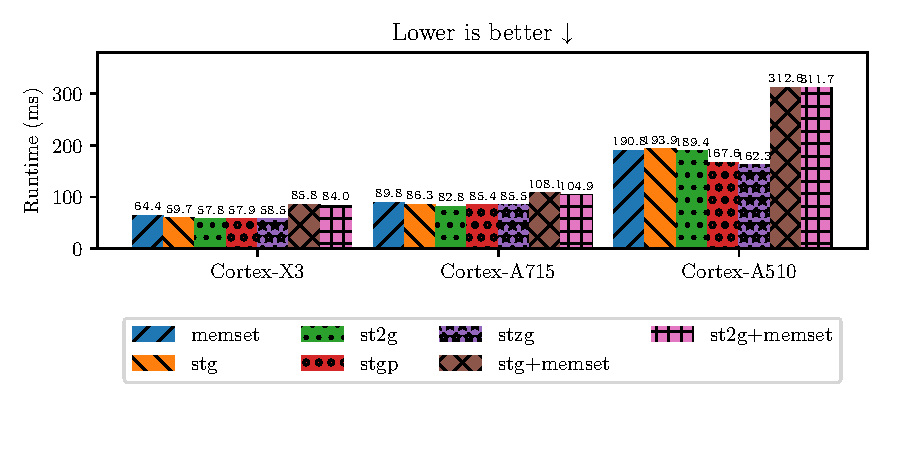
\includegraphics{plots/stg}
    \caption{Performance results of the benchmarking variants from \cref{tab:stg-instructions} on 128\,MiB of memory.}
    \label{fig:stg-performance}
\end{figure}

We perform all runs on each type of CPU core on the Pixel 8 and illustrate the results in \cref{fig:stg-performance}.
As expected, the instructions implicitly setting the memory to zero are faster than tagging and then zeroing using an explicit memset.
Both \texttt{stzg} and \texttt{stgp} are only slightly slower than a raw memset, as their memory accesses do not need to perform tag checks~\cite{ARMA2024Arch64}.

Contrary to our expectations, \texttt{st2g} is only marginally faster than \texttt{stg}.
This finding contradicts the data presented in \cref{subsec:instruction-latencies-and-throughput}, where operations are performed with pre-filled data caches.
In these benchmarks, we specifically measure wall clock time, not processor cycles, to evaluate performance when tagging a large region of memory immediately after requesting it from the operating system.
This approach involves requesting a fresh segment of memory before each execution.
The Cortex-X3 achieves shorter execution times than the Cortex-A720, despite us measuring lower instructions executed per cycle, due to its higher clock speed.

\subsection{Synchronous and Asynchronous Mode}
\label{subsec:synchronous-and-asynchronous-mode}

We evaluate the performance of sequential memory accesses with \ac{MTE} disabled and enabled using synchronous mode and asynchronous mode on each type of CPU core on the Pixel 8.
This represents the raw overhead of enabling \ac{MTE} without additional instructions.
In \cref{fig:sync-async-performance}, we see that with synchronous mode, \texttt{memset} is 11.5\%, 8.9\%, and 13.2\% slower on the respective cores compared to the baseline with \ac{MTE} disabled.
Asynchronous mode is closer to the baseline with an overhead of 0.9\%, 3.7\%, and 6.1\% respectively.

\begin{figure}[h]
    \centering
    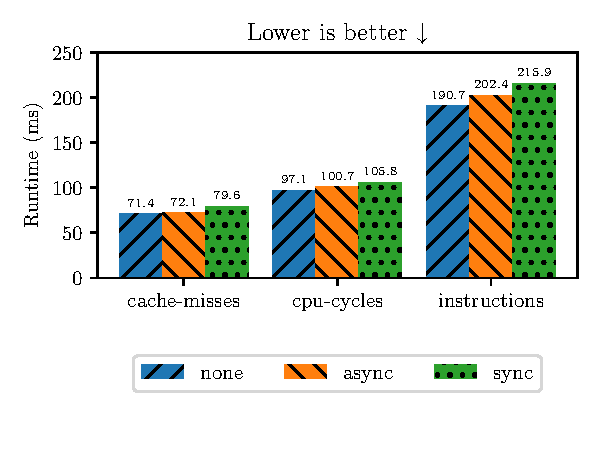
\includegraphics{plots/sync-async}
    \caption{Runtime of \texttt{memset} on 128\,MiB of memory using different \ac{MTE} modes.}
    \label{fig:sync-async-performance}
\end{figure}

\subsection{Migrating Tagged Memory}
\label{subsec:migrating-tagged-memory}

Migrating tagged memory involves the coordinated transfer of both data and its associated tags.
In \cref{fig:migrate-performance}, we analyze the performance of two migration strategies.

\begin{enumerate}
    \item Baseline (\texttt{memcpy} with \ac{MTE}): This baseline establishes the cost of a standard memory copy operation with \ac{MTE} enabled.
    \item \ac{MTE} Disable/Re-enable: Disabling \ac{MTE}, copying data with \texttt{memcpy}, transferring tags, and re-enabling \ac{MTE}.
    This method temporarily compromises memory safety during the transfer if other threads rely on \ac{MTE} being active during this approach.
    \item Iterative Copying: Copying tags and data in 16\,byte granules allows copying tags and data simultaneously while keeping \ac{MTE} active for other threads.
\end{enumerate}

Approach 3 is slightly slower than approach 2 on the Cortex-X3 but faster on the other cores.

\begin{figure}[h]
    \centering
    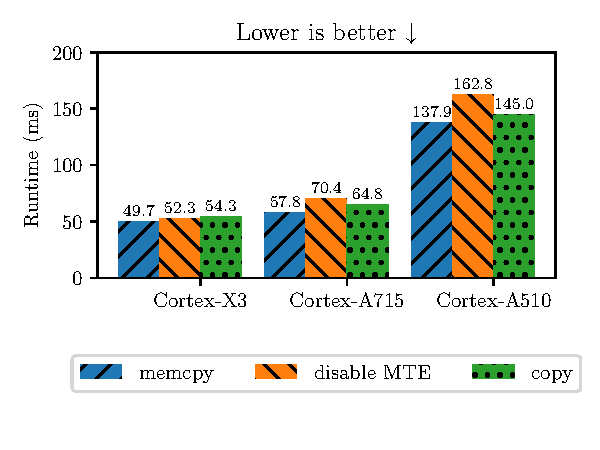
\includegraphics{plots/migrate}
    \caption{Runtime comparison of strategies for moving 128 MiB of memory and tags between regions.}
    \label{fig:migrate-performance}
\end{figure}

    \chapter{Related Work}
\label{ch:related}

\section{Memory Safety for WebAssembly}
\label{sec:related-memory-safety-for-webassembly}

This thesis builds upon existing efforts in the field of memory safety for \ac{WASM}.
Here, we examine notable projects aiming to achieve similar goals and highlight the distinct contributions of our research.

\subsection{MS-WASM}
\label{subsec:ms-wasm}

A significant project in this domain is MS-WASM, a memory safety extension for WASM introduced by \citeauthor*{disselkoen2019position} and further developed by \citeauthor*{michael2023mswasm}~\cite{disselkoen2019position,michael2023mswasm}.
MS-WASM introduces a new \textit{segment memory} distinct from the linear memory, preventing accesses through arbitrary offsets.
The segment memory relies on access through unforgeable \textit{handles}, akin to CHERI pointers~\cite{woodruff2014cheri}.

\paragraph{Key Differences}
This thesis adopts a different approach by enabling a gradual migration of memory segments into the linear memory.
This preserves compatibility with unmodified code, as only the allocation of memory regions has to be changed.
Memory accesses are still performed through integers, not pointers.
We do not implement intra-memory safety to allow implementation with \ac{MTE}, which uses colors for memory access control rather than the shading required for intra-object safety.
Utilizing \ac{MTE} allows our implementation to run with significantly lower overhead on devices supporting this technology.

\subsection{RichWasm}
\label{subsec:richwasm}

RichWasm is a richly-typed intermediate language designed to facilitate safe memory interactions between languages with diverse memory management models (e.g., manual and garbage-collected)~\cite{paraskevopoulou2024richwasm}.
It enables static detection of potential memory safety violations, making it particularly valuable for mixed-language interoperability.

RichWasm is intended for use as a compilation target for safe languages like Rust or OCaml, which have strong memory safety guarantees encoded in their type systems.
Languages like C, which lack information for static type safety analysis, are not directly supported by RichWasm's type-driven safety model.

\subsection{Pointer Authentication}
\label{subsec:related-pointer-authentication}

\citeauthor*{rehde2023wasm} has worked on implementing pointer authentication primitives~\cite{rehde2023wasm}.
In their work, they add pointer authentication primitives backed by ARM's \ac{PAC} to the memory safety extension described in this thesis.
This complements our work by providing additional protection mechanisms against pointer corruption.

\section{MTE for Memory Safety}
\label{sec:mte-for-memory-safety}

A few memory allocators have implemented support for MTE, including:

\begin{itemize}
    \item Scudo Hardened Allocator (used in Android): A security-oriented allocator providing defense mechanisms against heap-based vulnerabilities\footnote{\url{https://llvm.org/docs/ScudoHardenedAllocator.html}}.
    \item Chrome's PartitionAlloc: A partitioning allocator focusing on security and efficiency for multithreaded environments\footnote{\url{https://chromium.googlesource.com/chromium/src/+/master/base/allocator/partition_allocator/}}
    \item glibc's Ptmalloc: The GNU C library's standard memory allocator, with evolving experimental support for MTE\footnote{\url{https://ftp.gnu.org/gnu/glibc/}}.
\end{itemize}

\section{Memory Safety}
\label{sec:related-memory-safety}

Additionally, an overview of other important projects contributing to memory safety:

\subsection{ASAN}
\label{subsec:related-asan}

\ac{ASAN} is a compiler instrumentation tool that dynamically detects memory safety errors at runtime~\cite{serebryany2012addresssanitizer}.
It employs techniques like shadow memory to track memory states and flag heap and stack overflows, use-after-free errors, use-after-return errors, and other memory-related issues.

\ac{ASAN} is widely used in development and testing environments due to its effectiveness but is usually not deployed in production due to its runtime overhead.

\subsection{GWP-ASan}
\label{subsec:gwp-asan}

GWP-ASan adopts a probabilistic approach to memory safety~\cite{serebryany2023gwp}.
It samples a subset of allocations and places them in a guarded memory region to detect spatial and temporal memory safety violations for those allocations.

The low selection probability means GWP-ASAN has minimal runtime overhead, making it suitable for large-scale production deployments.
Its goal is to identify hard-to-reproduce memory bugs triggered by real-world user behavior and not covered by fuzzing or tests.

    \chapter{Conclusion}
\label{ch:conclusion}

In this thesis, we presented three pieces of work:
(1) a minimally-invasive and adaptable \ac{WASM} extension to provide memory safety primitives to compilers and programmers,
(2) an implementation consisting of (2a) a compiler toolchain integrated into LLVM, including a modified wasi-libc and allocator to provide spatial and temporal memory safety for the heap, an LLVM sanitizer pass to instrument stack allocations,
(2b) an implementation in wasmtime, compiling and running the \ac{WASM} extension on \ac{MTE} hardware, and utilizing \ac{MTE} as a replacement for software-based bounds checks,
and (3) an evaluation of our work and \ac{MTE} on real hardware.

\section{Future Work}
\label{sec:future-work}

\subsection{Additional Implementations}
\label{subsec:additional-implementations}

We have implemented a prototype based on \ac{MTE} for our memory safety extension.
However, additional implementations exploring different extensions, such as ARM's \ac{TBI}, available from ArmV8.0, would allow storing metadata in the top byte while performing access checks in software, similar to \ac{HWASAN}~\cite{serebryany2018memory}.
Software-based implementations, while slower, would allow deploying the memory safety extension to more devices than possible using recent extensions, such as \ac{MTE}.

We are working on an implementation utilizing \ac{CHERI}, with an in-progress implementation for the ARM Morello development board~\cite{UCAM-CL-TR-982}.
The CHERI architecture provides much more fine-grained checks and unlimited compartments but requires widening pointers to 128\,bits and moving from a fixed 16\,byte alignment for segments to a dynamic alignment, depending on the size of the segment.
Additionally, revoking capabilities for temporal memory safety is more involved compared to \ac{MTE}~\cite{xia2019cherivoke}, where memory can just be retagged.
Exploring and comparing these tradeoffs will be part of our future work.

\subsection{Backward Compatibility}
\label{subsec:backward-compatibility}

Currently, code compiled with the memory safety extension requires a modified runtime aware of this extension.
We are exploring techniques to embed metadata about allocations in custom \ac{WASM} segments that are ignored by runtimes but are used to provide memory safety when running on a modified runtime.

\subsection{Combining Guard Pages and \ac{MTE}}
\label{subsec:combining-guard-pages-and-mte}

Currently, we are limiting the number of sandboxes to 15, as we allocate the zero tag for the runtime and one tag per instance.
Future work might explore possibilities to increase the number of sandboxes by combining \ac{MTE} with guard pages.

\subsection{Pointer Authentication}
\label{subsec:future-work-pac}

In a previous Bachelor's thesis, \citeauthor{rehde2023wasm} explored the integration of pointer authentication primitives for data pointers to the \ac{WASM} extension, with an implementation using ARM's \ac{PAC} extension~\cite{rehde2023wasm}.
While \ac{WASM} lacks raw function pointers, table indices remain vulnerable to overwriting and forgery.
As we do not support intra-object safety, some overflow exploits remain possible.
These could, for instance, target an objects virtual function table to redirect control flow to a different function.

By adding support for data pointers to sign and authenticate these table indices, we would provide another layer of defenses against some attacks.


    \appendix{}

    \chapter{Artifacts}
\label{ch:artifacts}

The artifacts are available on GitHub.
They consist of the following repositories:

\begin{itemize}
    \item LLVM: \url{https://github.com/TUM-DSE/llvm-memsafe-wasm}
    \item wasmtime: \url{https://github.com/TUM-DSE/wasmtime-mte}
    \item wasm-tools: \url{https://github.com/TUM-DSE/wasm-tools-mte}
    \item wasi-sdk: \url{https://github.com/martin-fink/wasi-sdk}
    \item wasi-libc: \url{https://github.com/martin-fink/wasi-libc}
    \item PolyBench/C: \url{https://github.com/martin-fink/polybench-c}
\end{itemize}

\section{Building}
\label{sec:building}

All the projects contain a \texttt{flake.nix} that can be used to start a development shell containing all the dependencies.
These need to be installed manually on systems without Nix.

\subsection{LLVM Toolchain}
\label{subsec:llvm-toolchain}

The following commands can be used to bootstrap the \ac{WASM} compiler toolchain, including the libc.

\begin{lstlisting}[label={lst:building-sdk}]
    git clone --recurse-submodules https://github.com/martin-fink/wasi-sdk.git
    cd wasi-sdk
    make package
    cd dist
    tar -xzf wasi-sdk-20.38g2b3e8f68d320-linux.tar.gz
    tar -xzf libclang_rt.builtins-wasm64-wasi-20.38g2b3e8f68d320.tar.gz
    mv lib wasi-sdk-20.38g2b3e8f68d320/lib/clang/18/
\end{lstlisting}

\subsection{Wasmtime}
\label{subsec:building-wasmtime}

We are building wasmtime for Android, as the Pixel 8 is the only device supporting \ac{MTE} at the time of writing.
The same steps are also possible if you are building for Linux.
In any case, you need a C compiler and linker for the corresponding target.

\begin{lstlisting}[label={lst:building-wasmtime}]
    git clone --recurse-submodules \
        https://github.com/TUM-DSE/wasmtime-mte.git wasmtime
    cd wasmtime
\end{lstlisting}

\subsubsection{Building for Android}

You need to install the Android NDK\footnote{\url{https://developer.android.com/ndk}} to compile wasmtime for Android.
The resulting binary will be placed in \texttt{./target/aarch64-linux-android/release/wasmtime}.

\begin{lstlisting}[label={lst:configuring-wasmtime-android}]
    rustup target add aarch64-linux-android
    mkdir .cargo
    echo << EOF
    [env]
    [target.aarch64-linux-android]
    linker = "/path/to/android/aarch64-linux-android34-clang"
    ar = "/path/to/android/llvm-ar"
    rustflags = ["-C", "target-feature=+mte"]
    EOF >> .cargo/config.toml
    cargo build --release --target aarch64-linux-android
\end{lstlisting}

\subsubsection{Building for Linux}

You need a cross-compiler for aarch64 Linux.
The resulting binary will be placed in \texttt{./target/aarch64-unknown-linux-gnu/release/wasmtime}.

\begin{lstlisting}[label={lst:configuring-wasmtime-linux}]
    rustup target add aarch64-unknown-linux-gnu
    mkdir .cargo
    echo << EOF
    [env]
    CC_aarch64-unknown-linux-gnu = "aarch64-linux-gnu-gcc"
    CC_aarch64-unknown-linux-musl = "aarch64-linux-gnu-gcc"

    [target.aarch64-unknown-linux-gnu]
    linker = "aarch64-linux-gnu-gcc"
    rustflags = ["-C", "target-feature=+mte"]

    [target.aarch64-unknown-linux-musl]
    linker = "aarch64-linux-gnu-gcc"
    rustflags = ["-C", "target-feature=+mte"]
    EOF >> .cargo/config.toml
    cargo build --release --target aarch64-unknown-linux-gnu
\end{lstlisting}

\section{Running Programs}
\label{sec:running-programs}

\subsection{Compiling with Memory Safety}\label{subsec:compiling-with-memory-safety}

LLVM supports the flags described in \cref{tab:llvm-flags}.

\begin{lstlisting}[label={lst:compiling-to-wasm}]
    WASI_SDK=wasi-sdk-20.38g2b3e8f68d320
    "./$WASI_SDK/bin/clang" \
      -mmem-safety \
      -Os \
      -fsanitize=wasm-memsafety \
      --sysroot "$WASI_SDK/share/wasi-sysroot" \
      main.c \
      -o main.wasm
\end{lstlisting}

\subsection{Running with Wasmtime}\label{subsec:running-with-wasmtime}

Copy the wasmtime binary built in \cref{subsec:building-wasmtime} to an \ac{MTE}-capable device, e.g., QEMU.
Wasmtime supports the flags described in \cref{tab:wasmtime-flags}.

\begin{lstlisting}[label={lst:running-wasm}]
    ./wasmtime run \
      -W memory64 \
      -W mem-safety \
      -C mte-bounds-checks \
      -C mte \
      main.wasm
\end{lstlisting}


    \microtypesetup{protrusion=false}

    \addchap{Abbreviations}
    \begin{acronym}
        \itemsep-.25\baselineskip
        \acro{ASAN}[ASan]{Address Sanitizer}
        \acro{CHERI}[CHERI]{Capability Hardware Enhanced RISC Instructions}
        \acro{CLIF}[CLIF]{Cranelift IR}
        \acro{GEP}[GEP]{\texttt{getelementptr}}
        \acro{HWASAN}[HWASan]{Hardware-Assisted Address Sanitizer}
        \acro{IR}[IR]{intermediate representation}
        \acro{ISA}[ISA]{instruction set architecture}
        \acro{MMU}[MMU]{Memory Management Unit}
        \acro{MTE}[MTE]{Memory Tagging Extension}
        \acro{PAC}[PAC]{Pointer Authentication}
        \acro{ROP}[ROP]{return-oriented programming}
        \acro{rss}[rss]{resident set size}
        \acro{TBI}[TBI]{Top Byte Ignore}
        \acro{WASI}[WASI]{WebAssembly System Interface}
        \acro{WASM}[WASM]{WebAssembly}
    \end{acronym}

    \listoffigures{}
    \listoftables{}
    \microtypesetup{protrusion=true}
    \printbibliography{}

\end{document}
